\documentclass[11pt,a4paper]{article}

\usepackage[utf8]{inputenc}
\usepackage[T1]{fontenc}
\usepackage[margin=2.5cm]{geometry}
\usepackage{amsmath,amssymb}
\usepackage{graphicx}
\usepackage{booktabs}
\usepackage{array}
\usepackage{xcolor}
\usepackage{hyperref}
\usepackage{enumitem}
\usepackage{titlesec}
\usepackage{parskip}
\usepackage{caption}

\definecolor{frcblue}{RGB}{28,45,68}
\definecolor{frcaccent}{RGB}{18,118,150}

% Tighter float-packing so figure-dense appendix pages don't leave large
% blank areas below a single figure (does not affect body-text pages).
\renewcommand{\topfraction}{0.95}
\renewcommand{\textfraction}{0.02}
\renewcommand{\floatpagefraction}{0.75}
\setlength{\floatsep}{6pt plus 2pt minus 2pt}
\setlength{\textfloatsep}{8pt plus 2pt minus 2pt}
\setlength{\intextsep}{6pt plus 2pt minus 2pt}

\titleformat{\section}{\normalfont\Large\bfseries\color{frcblue}}{\thesection}{1em}{}
\titleformat{\subsection}{\normalfont\large\bfseries\color{frcblue}}{\thesubsection}{1em}{}
\titleformat{\subsubsection}{\normalfont\normalsize\bfseries}{\thesubsubsection}{1em}{}

\hypersetup{
  colorlinks=true,
  linkcolor=frcaccent,
  citecolor=frcaccent,
  urlcolor=frcaccent,
  pdftitle={Motion Planning and INDI for Aggressive Quadrotor Trajectory Tracking},
  pdfauthor={Georg Wolnik}
}

\newcommand{\code}[1]{\texttt{#1}}

\title{\color{frcblue}Motion Planning and Incremental Nonlinear Dynamic Inversion\\
for Aggressive Quadrotor Trajectory Tracking\\
on the Crazyflie 2.x Platform Family}
\author{Georg Wolnik \\ \small Advanced Flying Robots \\
\small Supervisor: Prof.\ Wolfgang H\"onig \\ \small Mentor: Omar Elsayed (partially Khaled Wahba)}
\date{}

\begin{document}

\maketitle

\begin{abstract}
This report describes the design, implementation, and experimental evaluation of a full
autonomous-flight stack: minimum-snap motion planning with automatic time allocation, a
differential-flatness-based geometric SE(3) baseline controller, and an Incremental Nonlinear
Dynamic Inversion (INDI) attitude controller. All three components were deployed and compared
across three quadrotor platforms: a standard Crazyflie 2.1, a thrust-upgraded Crazyflie 2.1, and a
Crazyflie 2.1 Brushless (CF21BL). Each platform was commissioned end-to-end (motor identification
via RPM, filter tuning, cascaded gain tuning) and evaluated on a shared figure-8 tracking
benchmark, plus oval and circle trajectories swept across a range of planner aggressiveness. The
main result is a controller-and-platform comparison showing that full INDI reduces XY tracking
RMSE by 37--60\% relative to the geometric SE(3) baseline. The brushless platform's higher motor
bandwidth ($\tau\approx44$\,ms vs.\ 71\,ms for the thrust-upgraded platform) allows more aggressive
attitude gains and gives the best overall tracking performance (2.45\,cm mean RMSE, $n=13$), but
also brings a resonant $\approx7.2$\,Hz attitude oscillation that the thrust-upgraded platform's
lower bandwidth avoids. We trace the root cause of this oscillation (closed-loop resonance at
$\omega_n=\sqrt{K_R}$, with actuator lag as the dominant and EKF attitude-estimate lag as a
secondary phase-loss term) and design a targeted band-reject (notch) filter as a fix; it is
implemented and build-verified but has not yet been flight-tested. The remaining sections cover
related work, the planning and control methods used, the experimental setup, the results, a
discussion of the cross-platform differences, and the project's open limitations.
\end{abstract}

%======================================================================
\section{Introduction}
%======================================================================

Tracking aggressive trajectories accurately relies on two complementary techniques. The first is
\textbf{differential-flatness-based motion planning}, which produces dynamically feasible,
minimum-effort trajectories together with closed-form full-state references derived directly from
the position trajectory and its derivatives. The second is \textbf{Incremental Nonlinear Dynamic
Inversion (INDI)}, a control technique that replaces an explicit dynamics model with a real-time
measurement of the vehicle's actual angular acceleration, so the attitude loop stays robust to
unmodeled effects and platform-specific uncertainty.

This project implements both. A minimum-snap planning pipeline with automatic time allocation
(Richter et al.~\cite{richter2016}) generates the trajectories, and full INDI attitude control
(Tal \& Karaman~\cite{tal2020}), including the RPM-feedback-based torque estimation it requires,
tracks them on real Crazyflie hardware. We commissioned the full stack end to end (motor
identification via RPM, filter tuning, cascaded gain tuning) on three physical platforms: a
standard, a thrust-upgraded, and a brushless CF21BL Crazyflie 2.x. This lets us see how
platform-specific actuator dynamics limit the achievable control bandwidth and tracking accuracy.
Each platform is benchmarked against a common geometric SE(3) baseline and pushed across a
planner-aggressiveness sweep ($k_t$) to find its practical ceiling.

Two originally planned phases were dropped once a data-confirmed attitude resonance on the
highest-bandwidth platform became the project's main open question
(Section~\ref{sec:shake-root-cause}): commissioning a third platform, and a dedicated accel-pinned
aerobatics phase. Part of that aerobatics work, a fully inverted loop, was still completed as
bonus work once time allowed (Section~\ref{sec:limitations}). It uses a separate,
explicit-attitude planning approach that is not one of the two automatic-time-allocation planning
modes used for every other experiment in this report (Section~\ref{sec:planning-methods}).

%======================================================================
\section{Related Work}
%======================================================================

A quadrotor's translational dynamics are differentially flat~\cite{mellinger2011}: the full 6-DOF
state and the control inputs can be written as algebraic functions of the position trajectory
$\mathbf{p}(t)$, yaw $\psi(t)$, and a finite number of their derivatives (up to snap for the full
state, one derivative further for angular-acceleration feedforward). A smooth polynomial in
position/yaw space is therefore enough to derive a complete, dynamically consistent reference
without ever planning attitude directly. Our baseline attitude controller follows the geometric
SE(3) approach of Lee et al.~\cite{lee2010}, which computes attitude and rate errors directly on
SO(3), avoiding the singularities of an Euler-angle representation, and commands torque
model-based from these errors plus a gyroscopic decoupling term. Trajectories are generated with
Mellinger and Kumar's~\cite{mellinger2011} minimum-snap QP formulation, extended by Richter et
al.~\cite{richter2016} to automate per-segment timing from a single aggressiveness scalar $k_t$.
The INDI attitude law (Tal \& Karaman~\cite{tal2020}) replaces the geometric law's model-based
feedback with an incremental update: the next torque command is the currently applied torque plus
a correction proportional to the gap between the desired and the measured angular acceleration.
Because any unmodeled effect shows up directly in that measurement, INDI stays robust to model
mismatch without needing the mismatch to be characterized in advance. This property turns out to
matter a great deal for the main practical challenge of this project
(Section~\ref{sec:shake-root-cause}).

%======================================================================
\section{Methods}
%======================================================================

\subsection{Motion planning}
\label{sec:planning-methods}

All trajectories in this project are generated by one of two automatic-time-allocation planning
modes. Both are built on the same minimum-snap QP machinery (\code{src/planning/richter.rs}) and
both are driven by a single scalar aggressiveness parameter $k_t$ rather than manually chosen
segment durations:

\begin{itemize}
  \item \textbf{Mode~1} (\code{RichterTrajectory::plan()}) uses Richter et al.'s~\cite{richter2016}
    time-allocation formula,
    \[
      T_i = \max\!\left(\frac{\mathrm{dist}_i}{v_{\mathrm{avg}}(k_t)},\, T_{\min}\right),
      \qquad v_{\mathrm{avg}} = 0.5 + 1.5\sqrt{k_t}, \qquad T_{\min}=0.15\,\mathrm{s}
    \]
    below which the QP's $1/T^7$ segment weighting becomes numerically degenerate. We use zero
    redistribution iterations by default, favoring robustness and predictability over the
    marginal timing refinement the full paper formulation offers.
  \item \textbf{Mode~3} (\code{RichterTrajectory::plan\_paper()}) uses the same time-allocation
    formula but adds the full eight gradient-descent redistribution iterations specified in
    Richter et al.~\cite{richter2016}, which push segment time toward the highest-snap portions
    of the trajectory for more balanced actuator demand across the maneuver.
\end{itemize}

Both modes share the same differential-flatness recovery, following the Faessler et
al.~\cite{faessler2018} formulation (implemented in \code{src/planning/flatness.rs}). Given the
position polynomial's derivatives at any query time $t$ (velocity, acceleration, jerk, snap) plus
yaw and its derivatives, the full rigid-body reference is recovered in closed form:

\begin{align}
  \mathbf{a}_g &= \ddot{\mathbf{p}} + g\hat{\mathbf{z}} \\
  \mathbf{x}_b &= \mathrm{normalize}(\mathbf{y}_c \times \mathbf{a}_g), \quad
  \mathbf{y}_b = \mathrm{normalize}(\mathbf{a}_g \times \mathbf{x}_b), \quad
  \mathbf{z}_b = \mathbf{x}_b \times \mathbf{y}_b \\
  c &= \mathbf{z}_b \cdot \mathbf{a}_g, \qquad T = m\,c \\
  \boldsymbol{\omega} &= f(\mathbf{j}, \mathbf{x}_b, \mathbf{y}_b, c)
    \qquad \text{(from jerk } \mathbf{j}=\dddot{\mathbf{p}}\text{)} \\
  \dot{\boldsymbol{\omega}} &= f(\mathbf{s}, \boldsymbol{\omega}, \mathbf{x}_b, \mathbf{y}_b, c)
    \qquad \text{(from snap } \mathbf{s}=\mathbf{p}^{(4)}\text{)} \\
  \boldsymbol{\tau} &= J\dot{\boldsymbol{\omega}} - (J\boldsymbol{\omega})\times\boldsymbol{\omega}
\end{align}

Here $\mathbf{x}_c = [\cos\psi, \sin\psi, 0]$ and $\mathbf{y}_c = [-\sin\psi, \cos\psi, 0]$ define
the yaw-heading intermediate frame used to disambiguate the body-$x$/body-$y$ axes from the
thrust-direction-only $\mathbf{z}_b$. This closed-form map lets the entire trajectory library used
in this project (figure-8, circle, oval, corner, helix, tilted oval) be authored purely as
position/yaw waypoints. Attitude, angular rate, angular acceleration, and thrust are all derived
from that, never planned separately.

\subsection{Geometric SE(3) baseline control}

The geometric controller~\cite{lee2010} is the same control law used across all three platforms
and is INDI's structural baseline throughout this report. The formal, validated geometric-vs-INDI
comparison in Section~5.2 (Table~1) was carried out on the standard platform only; the
thrust-upgraded and brushless platforms are compared to each other and to that standard-platform
reference through their own INDI results, not through their own separate geometric campaigns.
Attitude error is computed on SO(3):
\[
  \mathbf{e}_R = \tfrac{1}{2}\,\mathrm{vee}\!\left(R_d^\top R - R^\top R_d\right)
\]
and torque is commanded directly from a model-based law:
\[
  \boldsymbol{\tau} = -K_R \mathbf{e}_R - K_W \mathbf{e}_\omega + \boldsymbol{\omega}\times J\boldsymbol{\omega}
\]
with $K_R$ and $K_W$ tuned per platform (the position loop uses $K_P$/$K_V$ on position/velocity
error with the same cascade structure). Because this law is purely model-based, its accuracy
depends on how closely $J$ (inertia) and the thrust/torque allocation model match the real
airframe.

\subsection{INDI attitude control}

The INDI attitude law, following Tal \& Karaman~\cite{tal2020} directly, replaces the geometric
law's model-based torque computation with four coupled equations.

\subsubsection{(1) Feedforward}

The desired angular acceleration $\boldsymbol{\alpha}_{\mathrm{des}}$ is computed from the
trajectory's snap via differential flatness (Tal \& Karaman~\cite{tal2020}, Eq.~15). This is the
only place the desired trajectory's higher derivatives feed the attitude loop; everything else
below is feedback.

\subsubsection{(2) Reference blend}

\[
  \boldsymbol{\alpha}_{\mathrm{ref}} = \boldsymbol{\alpha}_{\mathrm{des}}
    - K_R \mathbf{e}_R - K_W \mathbf{e}_\omega \qquad \text{(Eq.~28)}
\]
This has the same form as the geometric law's gains, but $\boldsymbol{\alpha}_{\mathrm{ref}}$ is a
desired acceleration, not a torque. $K_R$ has units $1/\mathrm{s}^2$ (closed-loop bandwidth
$\omega_n=\sqrt{K_R}$) and $K_W$ has units $1/\mathrm{s}$ (damping ratio $\zeta=K_W/(2\omega_n)$).

\subsubsection{(3) Measured angular acceleration}

No sensor measures angular acceleration directly, so $\boldsymbol{\alpha}_{\mathrm{meas}}$ is
derived from the gyroscope through a two-stage chain, matching the order specified by Tal \&
Karaman~\cite{tal2020} Sec.~III-D and the stock Crazyflie firmware: the raw body rate is first
low-pass filtered, then differentiated.
\[
  \boldsymbol{\omega}_{\mathrm{filt}}[k] = \mathrm{BW}(\boldsymbol{\omega}_{\mathrm{raw}}[k]),
  \qquad
  \boldsymbol{\alpha}_{\mathrm{meas}}[k] =
    \frac{\boldsymbol{\omega}_{\mathrm{filt}}[k]-\boldsymbol{\omega}_{\mathrm{filt}}[k-1]}{\Delta t}
\]
The same Butterworth filter is applied identically to $\boldsymbol{\alpha}_{\mathrm{ref}}$, which
keeps the reference and measured legs phase-matched before their difference is taken in the
increment law below.

\subsubsection{(4) Incremental torque law}

\begin{align}
  \delta\boldsymbol{\tau} &= J\left(\boldsymbol{\alpha}_{\mathrm{ref}} - \boldsymbol{\alpha}_{\mathrm{meas}}\right) \\
  \boldsymbol{\tau}_{\mathrm{new}} &= \boldsymbol{\tau}_{\mathrm{current}} + \delta\boldsymbol{\tau}
    \qquad \text{(Eq.~31)}
\end{align}

This is the core INDI mechanism: a small correction to whatever torque is currently applied,
using measured, not modeled, angular acceleration. $\boldsymbol{\tau}_{\mathrm{current}}$ is
estimated from the physical system, per-motor RPM converted to thrust via a bench-identified motor
constant $k_T$ and then mapped to body torque via the known arm geometry, rather than from the
previous commanded torque, which would not account for real motor response lag. This is the key
structural difference from the geometric law: INDI does not need an accurate model of
thrust-to-RPM response, aerodynamic drag, or other unmodeled disturbances, because any such effect
already shows up in $\boldsymbol{\alpha}_{\mathrm{meas}}$ and is rejected by the increment on the
next cycle.

\subsection{An added filter stage: targeting a diagnosed narrowband resonance}
\label{sec:notch-methods}

Brushless-platform commissioning identified a narrowband attitude oscillation at
$\approx7.22$\,Hz (Section~\ref{sec:shake-root-cause} gives the full root-cause analysis). We
confirmed by 500\,Hz SD-card measurement that the Stage-1 Butterworth filter (cutoff 60--70\,Hz)
passes this frequency essentially unattenuated
($|\boldsymbol{\alpha}_{\mathrm{meas}}|/|\boldsymbol{\alpha}_{\mathrm{raw}}| = 1.000$), and that
lowering the cutoff into that band degrades tracking substantially, since a broad low-pass trades
off phase margin below its cutoff, not just at the resonant band. We designed a targeted fix
instead: an optional, runtime-tunable second-stage band-reject (notch) filter, an RBJ
Audio-EQ-Cookbook band-reject biquad ($Q=f_0/\mathrm{bw}$, default center 7.2\,Hz, bandwidth
5\,Hz, giving a 4.7--9.7\,Hz attenuated band). When enabled it is applied identically to
$\boldsymbol{\alpha}_{\mathrm{meas}}$, $\boldsymbol{\alpha}_{\mathrm{ref}}$, and
$\boldsymbol{\tau}_{\mathrm{current}}$, so no term of the INDI sum ends up phase-mismatched,
mirroring the Stage-1 Butterworth's own reasoning. It is disabled by default
(\code{notch\_en=0}, verified byte-identical to prior behavior when off) and is implemented and
build-verified but not yet flight-tested (Section~\ref{sec:limitations}).

%======================================================================
\section{Experimental Setup}
%======================================================================

We commissioned three platforms: a \textbf{standard} Crazyflie 2.1 (brushed 0716 motors, 36.4\,g,
$J_{xx}=J_{yy}=1.657\times10^{-5}\,\mathrm{kg\,m^2}$, used as the reference platform), a
\textbf{thrust-upgraded} Crazyflie 2.1 (brushed upgrade kit, 38.6\,g, similar inertia, higher peak
thrust per motor at 0.18\,N vs.\ 0.13\,N, but a heavier rotor), and a \textbf{brushless} CF21BL
(41.0\,g, $\mathrm{diag}(2.40,2.40,3.24)\times10^{-5}\,\mathrm{kg\,m^2}$~\cite{busetto2025}, the
highest motor bandwidth of the three, with DShot bidirectional telemetry). Full physical
parameters are listed in Appendix~\ref{sec:appendix-configs} (Table~\ref{tab:platforms}). Every
platform was bench-identified for its per-motor thrust constant $k_T$ (thrust stand, RPM sweep,
$k_T=\mathrm{thrust}/\mathrm{RPM}^2$) before any INDI flight.

Trajectories are generated offline in Rust (\code{export\_poly4d}), converted to an 8-coefficient
Poly4D representation, and uploaded via the Crazyswarm2 (CS2) ROS~2 framework. Position is
estimated from OptiTrack and fed to the onboard EKF. The onboard high-level commander evaluates
the uploaded polynomial at 1\,kHz and feeds the geometric or INDI attitude controller, running at
500\,Hz, through the standard Crazyflie firmware loop. This gives globally drift-free pose for
repeatable long-duration, high-speed flights.

The primary metric throughout is \textbf{phase-aligned XY position RMSE}: the flown path is
time-shifted to maximize cross-correlation with the planned path before computing RMSE, which
corrects for any constant commanded-vs-flown lag. Secondary metrics are roll/pitch tracking error
and, for stress-testing, per-axis gyro standard deviation as a proxy for attitude oscillation
severity. We classify a flight as a \textbf{crash} (used throughout Section~5.3 and
Appendix~\ref{sec:appendix-ktsweep}) when logged altitude dives well below the commanded
trajectory, which is physically impossible under controlled flight, and this is corroborated by a
simultaneous jump in gyro standard deviation. Both signals are unambiguous in the logged telemetry
and were cross-checked against each flight's own recording. All exported trajectories were
validated against a physically confirmed usable flight volume ($x{:}\pm1.2$\,m, $y{:}\pm2.5$\,m,
$z{:}0.5$--$1.8$\,m) by densely sampling every trajectory across the full $k_t$ range flown and
checking worst-case bounding boxes before any flight.

The core benchmark for every cross-platform, cross-controller comparison is a \textbf{figure-8} at
$k_t=0.05$ (lap $\approx6.9$\,s). Extended aggressiveness sweeps additionally use \textbf{oval} and
\textbf{circle} shapes at increasing $k_t$ to find each platform's practical ceiling.

%======================================================================
\section{Results}
%======================================================================

\subsection{Per-platform tuning summary}

Full locked-configuration tables (all gains, filters, and bench-identified thrust constants) are
in Appendix~\ref{sec:appendix-configs} (Tables~\ref{tab:standard-config}--\ref{tab:brushless-config}).

\textbf{Standard CF2.1.} A filter cutoff sweep found $\mathrm{fc\_bw}=70$\,Hz optimal (3.1\,cm
RMSE). The final configuration is $K_R=1050$, $K_W=87$ ($\omega_n\approx32.4\,\mathrm{rad/s}$),
$K_{P,xy}=40$, $K_{V,xy}=3.3$. Over 10 flights, INDI averaged \textbf{3.87\,cm} RMSE against
6.14\,cm for the geometric baseline, a 37\% reduction (Figure~\ref{fig:geo-vs-indi},
Appendix~\ref{sec:appendix-figures}).

\textbf{Thrust-upgraded CF2.1.} The attitude gain ladder found a hard ceiling at $K_R=603$
($\omega_n\approx24.6\,\mathrm{rad/s}$), well below the standard platform's 1050, despite the
upgrade kit's higher peak thrust (0.18\,N vs.\ 0.13\,N per motor). The final configuration is
$K_R=603$, $K_W=90$ ($\zeta\approx1.83$, $\tau_{\mathrm{slow}}=137$\,ms), $K_{P,xy}=40$,
$K_{V,xy}=8$. An 11-flight validation gave \textbf{3.72\,cm} mean RMSE (std 0.21), close to the
standard platform despite the lower achievable $K_R$.

\textbf{Brushless CF21BL.} This platform saw the most extensive tuning campaign of the three. A
coupled gain ladder ($K_R$, $K_W$, $K_P$, $K_V$ scaled together) improved RMSE monotonically up to
a hover-noise ceiling at $K_R\approx2400$--$2600$. Decoupled sweeps then showed that pulling $K_W$
and $K_V$ down independently of that ratio improved both RMSE and attitude error at the same
time, a real decoupling win rather than a tradeoff, because $K_W$ injects raw gyro noise directly
and linearly through $K_W\mathbf{e}_\omega$. The final configuration is $K_R=2400$, $K_W=170$
($\zeta\approx1.74$), $K_{P,xy}=64$, $K_{V,xy}=5$. A 12-flight validation gave \textbf{2.48\,cm}
mean RMSE (std 0.14), the best of any platform in this project.

\subsection{Headline cross-platform/cross-controller comparison}

\begin{table}[t]
\centering
\begin{tabular}{@{}lrrrr@{}}
\toprule
Configuration & $n$ & Mean XY RMSE & Std & vs.\ Standard Geometric \\
\midrule
Standard Geometric (baseline) & 10 & 6.14\,cm & 0.52 & --- \\
Standard INDI & 10 & 3.87\,cm & 0.24 & $-37\%$ \\
Upgraded INDI & 11 & 3.72\,cm & 0.21 & $-39\%$ \\
Brushless INDI (fc\_bw=60) & 12 & 2.48\,cm & 0.13 & $-60\%$ \\
\textbf{Brushless INDI (fc\_bw=70)} & \textbf{13} & \textbf{2.45\,cm} & \textbf{0.12} & \textbf{$-60\%$} \\
\bottomrule
\end{tabular}
\caption{Five-way headline comparison, figure-8 trajectory, $k_t=0.05$.}
\label{tab:headline}
\end{table}

The $\mathrm{fc\_bw}=60$ vs.\ 70\,Hz brushless columns are otherwise identical configurations, so
they isolate the filter cutoff's effect: the two means ($2.48\pm0.14$ vs.\ $2.45\pm0.12$\,cm) fall
well within one combined standard deviation of each other across the 20--100\,Hz range tested (we
did not run a formal significance test). This is consistent with this platform's tracking ceiling
being set by attitude gain, and the resonance it induces (Section~\ref{sec:shake-root-cause}),
rather than filter tuning. A bar-chart visualization (Figure~\ref{fig:5way}) and the full
per-flight breakdown of the best brushless flight (flown path, 3D attitude, INDI torque, and RPM
balance) are reproduced at full size in Appendix~\ref{sec:appendix-figures}
(Figures~\ref{fig:best-analysis}--\ref{fig:best-rpm}).

\subsection{Extended aggressiveness sweeps (upgraded vs.\ brushless)}
\label{sec:extended-sweeps}

Full per-$k_t$ data (XY/Z RMSE, roll/pitch/yaw error, max speed) for both sweeps is in
Appendix~\ref{sec:appendix-ktsweep} (Tables~\ref{tab:oval-ktsweep}--\ref{tab:circle-ktsweep}).

\textbf{Oval.} Both platforms flew cleanly up to $k_t\le0.3$--$0.4$. The upgraded platform
crashed consistently at $k_t=0.5$--$0.6$ (3/3 attempts), while brushless stayed clean through
$k_t=0.5$ and crashed only at $k_t=0.7$. Brushless's working ceiling is roughly $k_t\approx0.5$
against upgraded's $k_t\approx0.3$--$0.4$. This tracks the bandwidth gap between them
($\omega_n\approx7.8\,\mathrm{Hz}$ for brushless vs.\ $\approx3.9\,\mathrm{Hz}$ for upgraded),
which gives brushless more control authority to correct through sharp direction changes, at the
cost of sitting closer to its own resonant regime.

\textbf{Circle.} This shape was newly swept on both platforms in this project; previously only
$k_t=0.05$ had been flown. Both platforms show the same pattern: a clean-flight region followed
by a marginal zone where crash and clean outcomes mix at the same $k_t$ rather than switching at
a sharp threshold. Upgraded stays clean to $\approx0.6$, brushless to $\approx0.5$, and both show
failures by $k_t=0.8$--$1.0$. Cross-platform RMSE at matched $k_t$ is tied at $k_t=0.05$ (1.7 vs.\
1.9\,cm) but favors brushless at $k_t=0.3$ (1.4 vs.\ 2.2\,cm, about 36\% lower), so which platform
tracks better depends on $k_t$ rather than being a fixed ranking.

Tracking-overview plots for both representative points (oval $k_t=0.4$, circle $k_t=0.7$) are
reproduced at full size in Appendix~\ref{sec:appendix-figures}
(Figures~\ref{fig:oval-kt04}--\ref{fig:circle-kt07}).

%======================================================================
\section{Discussion}
%======================================================================

\subsection{Why the platforms rank the way they do}

Considering position RMSE together with attitude tracking error gives a clearer ranking than
RMSE alone. In the best-flight breakdown (Appendix~\ref{sec:appendix-figures},
Figure~\ref{fig:best-analysis}), roll error runs $7.2^\circ$ (standard) $\to 5.3^\circ$
(upgraded) $\to 4.9^\circ$ (brushless), and pitch error $5.1^\circ \to 3.4^\circ \to 3.2^\circ$ in
the same order, with position RMSE following the same order in that flight (3.6, 3.2, 2.2\,cm).
So on both metrics, brushless tracks best, thrust-upgraded second, standard third, even though
the aggregate $n$-flight RMSE in Table~\ref{tab:headline} shows standard and upgraded close
enough (3.87 vs.\ 3.72\,cm) to fall within one combined standard deviation of each other.

Brushless's clear lead is well explained by achievable INDI attitude bandwidth, which is set by
motor response speed rather than peak thrust. Its bench-measured actuator time constant
($\tau\approx44$\,ms) is faster than the thrust-upgraded platform's ($\tau\approx71$\,ms), and
because INDI's stability margin depends on how quickly the motor can realize a commanded change
in angular acceleration, a faster actuator supports a higher stable $K_R$ (2400 vs.\ 603) and
therefore a higher closed-loop attitude bandwidth. This is a hardware-set advantage rather than a
tuning outcome. Brushless leads even with the $\approx7.22$\,Hz resonance below still unresolved;
fixing it should widen this lead, not shrink it.

The smaller gap between standard and upgraded does not fit the same explanation as cleanly: the
standard platform reaches a higher stable $K_R$ (1050 vs.\ 603) yet tracks slightly worse on
every metric above. We do not have a confirmed explanation for this reversal; it may reflect
differences elsewhere in the position or attitude loop rather than actuator bandwidth, and we
note it here rather than force a tidy story that the data does not fully support.

\subsection{The brushless attitude resonance: what we observed and our working hypothesis}
\label{sec:shake-root-cause}

Two things are directly observed, not inferred. First, the brushless platform's raw
angular-acceleration signal ($\alpha_{\mathrm{raw}}$) shows a narrowband spectral peak at
$\approx7.22$\,Hz, measured by 500\,Hz SD-card logging. The existing Stage-1 Butterworth filter
does essentially nothing to it ($|\mathrm{filtered}|/|\mathrm{raw}|=1.000$), since its cutoff
(60--70\,Hz) sits well above this band by design. Second, commanded torque on brushless is
markedly larger than on the other two platforms across all three axes in the same flight
comparison (Appendix~\ref{sec:appendix-figures}, Figure~\ref{fig:best-indi}): $\tau_z$ RMS is
2.17 vs.\ 0.19 (standard) and 0.14 (upgraded) N$\cdot$m, roughly an order of magnitude higher.

Beyond these two observations, what follows is our working hypothesis for the mechanism, not a
confirmed cause. Our leading candidate is a feedback resonance: $\omega_n=\sqrt{K_R}/2\pi =
7.80$\,Hz at $K_R=2400$ is close to the measured 7.22\,Hz peak (within 8\%), consistent with the
closed-loop attitude bandwidth sitting near its own resonant frequency and sustaining a
self-oscillation there, per the classical Barkhausen/Nyquist condition. Converting the
bench-measured actuator lag (31.6--33.6\,ms) to phase at 7.22\,Hz gives $\approx82^\circ$, about
four times the $\approx20^\circ$ from EKF attitude-estimate lag, so if this picture is right,
actuator lag is the larger of the two measured contributors. Lowering the filter cutoff into the
resonant band directly made tracking measurably worse, consistent with a low-pass trading off
phase margin across its whole passband to reach one narrow region. None of this proves the
mechanism; we have not, for example, varied $K_R$ independently over a wide enough range to
isolate it from other explanations. The full 500\,Hz diagnostic (hover and oval-maneuver spectra)
is in Appendix~\ref{sec:appendix-figures} (Figures~\ref{fig:shake-hover}--\ref{fig:shake-oval});
it shows the same peak at hover and under real maneuvering load.

Whatever the exact mechanism turns out to be, the two observations alone motivate the fix: a
narrowband energy peak sits in the signals that feed the INDI increment, and the existing filter
does not touch it. Removing that energy with a notch filter (Section~\ref{sec:notch-methods})
should reduce the oscillation it drives, whether or not our resonance explanation for why it
sits at 7.22\,Hz turns out to be fully correct.

%======================================================================
\section{Limitations \& Future Work}
\label{sec:limitations}
%======================================================================

\textbf{Brushless attitude resonance (open, pending validation).} The notch filter is
implemented and build-verified (byte-identical to prior behavior when disabled) but not yet
flight-tested. We expect a sharp amplitude drop in the notch-filtered signal at $\approx7$\,Hz
and calmer commanded torque; if the shake is instead dominated by actuator phase lag, this fix
may only partially resolve it. Other candidates considered but not pursued, since they need
hardware or firmware iteration beyond this project's scope: an actuator-lag compensation term in
the control law, reducing vibration at the source (prop balancing, mount damping), and,
speculatively, motor-protocol-level rate limiting (e.g.\ DShot slew-rate limiting).

\textbf{A separate crash} that was never root-caused occurred on a different maneuver, a wide
teardrop loop, under the plain geometric controller on both platforms at the mildest tested
aggressiveness. It was flagged but not investigated further.

\textbf{Inverted-loop aerobatic maneuver (bonus, beyond core scope).} Using a separate
explicit-attitude approach outside this report's core planning methods
(Section~\ref{sec:planning-methods}), we commissioned a fully inverted vertical loop on the
brushless platform: a repeatable inversion (roll $163$--$178^\circ$ at the apex, 3/3 flights) and,
in the best flight, a real post-inversion recovery. One narrower failure mode remains inside
the maneuver's auto-generated exit ramp. Several fixes were tried and ruled out; the mechanism is
well characterized but still unresolved.

\textbf{Third platform and dedicated aggressive-maneuver phase.} Both were descoped once the
resonance investigation became the dominant open question. The inverted-loop work above is a
partial, unplanned recovery of the latter.

%======================================================================
\section{Conclusion}
%======================================================================

This project implemented minimum-snap motion planning with automatic time allocation, a
differential-flatness-derived geometric baseline, and INDI attitude control, then commissioned and
evaluated all three on three physically distinct quadrotor platforms. The central result is a
37--60\% reduction in figure-8 tracking RMSE from INDI over the geometric baseline, governed almost
entirely by each platform's achievable motor bandwidth rather than by tuning effort. The
trajectory library was pushed beyond the core benchmark with oval and circle sweeps, which mapped
out real, platform-specific speed ceilings. The project's most significant open finding, a
narrowband $\approx7.22$\,Hz attitude resonance on the highest-bandwidth platform, is documented
with the observations behind it, a working hypothesis for its mechanism, and a data-driven fix, a
notch filter, that is implemented and ready for validation. Together with an unplanned excursion
into fully inverted aerobatic flight, the limitations reported here are, in every case,
well-characterized open problems rather than unexplained failures.

%======================================================================
\begin{thebibliography}{9}
%======================================================================

\bibitem{tal2020}
E.~Tal and S.~Karaman, ``Accurate Tracking of Aggressive Quadrotor Trajectories using
Incremental Nonlinear Dynamic Inversion and Differential Flatness,'' arXiv:1809.04048v2, 2020.

\bibitem{mellinger2011}
D.~Mellinger and V.~Kumar, ``Minimum snap trajectory generation and control for quadrotors,''
IEEE ICRA, 2011.

\bibitem{richter2016}
C.~Richter, A.~Bry, and N.~Roy, ``Polynomial trajectory planning for aggressive quadrotor
flight in dense indoor environments,'' in \textit{Robotics Research}, Springer, 2016.

\bibitem{lee2010}
T.~Lee, M.~Leok, and N.~H.~McClamroch, ``Geometric tracking control of a quadrotor UAV on
SE(3),'' IEEE CDC, 2010.

\bibitem{faessler2018}
M.~Faessler, A.~Franchi, and D.~Scaramuzza, ``Differential Flatness of Quadrotor Dynamics
Subject to Rotor Drag for Accurate Tracking of High-Speed Trajectories,'' IEEE RA-L, 2018.

\bibitem{busetto2025}
A.~Busetto et al., ``Nonlinear System Identification Nano-drone Benchmark,'' 2025 (brushless
platform parameters).

\end{thebibliography}

\clearpage
%======================================================================
\appendix
\section{Full INDI and Notch-Filter Equations}
\label{sec:appendix-equations}
%======================================================================

This appendix collects the complete equation set summarized in the Methods section, including
implementation-level detail (exact filter coefficients, the motor allocation matrix) omitted from
the main text for readability.

\subsection{Snap-based angular acceleration feedforward}

The desired angular acceleration $\boldsymbol{\alpha}_{\mathrm{des}}$ (Tal \& Karaman~\cite{tal2020}, Eq.~15) is
computed in closed form from the trajectory's jerk $\mathbf{j}=\dddot{\mathbf{p}}$ and snap
$\mathbf{s}=\mathbf{p}^{(4)}$, for constant yaw ($\dot\psi=0$):

\begin{align}
  \dot{c} &= \mathbf{b}_3\cdot\mathbf{j} \\
  \alpha_x &= \frac{2(\mathbf{y}_b\cdot\mathbf{j})(\mathbf{b}_3\cdot\mathbf{j})}{c^2}
    - \frac{\mathbf{y}_b\cdot\mathbf{s}}{c} \\
  \alpha_y &= \frac{\mathbf{x}_b\cdot\mathbf{s}}{c}
    - \frac{2(\mathbf{x}_b\cdot\mathbf{j})(\mathbf{b}_3\cdot\mathbf{j})}{c^2} \\
  \alpha_z &= 0
\end{align}

where $c=\|\mathbf{a}+g\hat{\mathbf{z}}\|$ and $\mathbf{x}_b,\mathbf{y}_b,\mathbf{b}_3$ are the
desired body axes from the flatness recovery (Section~\ref{sec:planning-methods}). This is a pure
feedforward term computed once per trajectory sample; no filtering is applied to
$\boldsymbol{\alpha}_{\mathrm{des}}$ itself, since it is a planned reference signal, not a noisy
measurement.

\subsection{Reference blend and rate error}

\begin{align}
  \mathbf{e}_\omega &= \boldsymbol{\omega} - \boldsymbol{\omega}_d \\
  \boldsymbol{\alpha}_{\mathrm{ref}} &= \boldsymbol{\alpha}_{\mathrm{des}}
    - K_R\,\mathbf{e}_R - K_W\,\mathbf{e}_\omega
\end{align}

where $\boldsymbol{\omega}_d$ (desired body angular rate) is itself a differential-flatness
feedforward term derived from jerk (Tal \& Karaman~\cite{tal2020}, Eq.~14), and $\mathbf{e}_R$ is the SO(3)
attitude error defined in Section~3.2.

\subsection{Measured angular-acceleration filter chain}

\textbf{Second-order Butterworth} (bilinear-transform biquad, cutoff $f_c$, sample period
$\Delta t$), applied to the raw body rate $\boldsymbol{\omega}_{\mathrm{raw}}$:
\[
  y[k] = b\big(x[k] + 2x[k-1] + x[k-2]\big) - a_1 y[k-1] - a_2 y[k-2]
\]
with the standard bilinear-transform coefficients $b$, $a_1$, $a_2$ derived from $f_c$ and
$\Delta t$.

\textbf{Finite difference}, applied to the filtered rate:
\[
  \boldsymbol{\alpha}_{\mathrm{meas}}[k] = \frac{\boldsymbol{\omega}_{\mathrm{filt}}[k]
    - \boldsymbol{\omega}_{\mathrm{filt}}[k-1]}{\Delta t}
\]

The identical Butterworth filter (same cutoff, independent instances) is applied to
$\boldsymbol{\alpha}_{\mathrm{ref}}$ to keep the reference and measured legs of the increment
phase-matched before their difference is taken in Eq.~A.5 below.

\subsection{Optional stage-2 notch (band-reject) filter}

The added filter of Section~\ref{sec:notch-methods} is a standard RBJ Audio-EQ-Cookbook
band-reject biquad, Direct Form~I, parameterized by center frequency $f_0$ and bandwidth
$\mathrm{bw}$ (both runtime-tunable):
\begin{align}
  \omega_0 &= 2\pi f_0 \Delta t, \qquad Q = \frac{f_0}{\mathrm{bw}} \\
  \alpha &= \frac{\sin\omega_0}{2Q}, \qquad a_0 = 1+\alpha \\
  b_0 = b_2 &= \frac{1}{a_0}, \qquad
  b_1 = a_1 = \frac{-2\cos\omega_0}{a_0}, \qquad
  a_2 = \frac{1-\alpha}{a_0} \\
  y[k] &= b_0 x[k] + b_1 x[k-1] + b_2 x[k-2] - a_1 y[k-1] - a_2 y[k-2]
\end{align}
With default $f_0=7.2$\,Hz, $\mathrm{bw}=5.0$\,Hz ($Q\approx1.44$), the $-3$\,dB attenuated band is
approximately $f_0\pm\mathrm{bw}/2 \approx 4.7$--$9.7$\,Hz, matching the diagnosed shake band.
When enabled, this same filter (independent instances, identical coefficients) is applied to
$\boldsymbol{\alpha}_{\mathrm{meas}}$, $\boldsymbol{\alpha}_{\mathrm{ref}}$, and the
increment-base term $\boldsymbol{\tau}_{\mathrm{current}}$ (Eq.~A.7 below), so that all three
terms entering the final torque command are attenuated identically at the resonant band.

\subsection{Incremental torque law and RPM-based increment base}

\begin{align}
  \delta\boldsymbol{\tau} &= J\left(\boldsymbol{\alpha}_{\mathrm{ref}}
    - \boldsymbol{\alpha}_{\mathrm{meas}}\right) \\
  \boldsymbol{\tau}_{\mathrm{new}} &= \boldsymbol{\tau}_{\mathrm{current}} + \delta\boldsymbol{\tau}
\end{align}

$\boldsymbol{\tau}_{\mathrm{current}}$ is estimated from measured per-motor RPM rather than the
previous commanded torque:
\begin{align}
  F_i &= k_{T,i}\cdot \mathrm{RPM}_i^2, \qquad i=1,\dots,4 \\
  \tau_x &= L\,(F_3+F_4-F_1-F_2) \\
  \tau_y &= L\,(F_2+F_3-F_1-F_4) \\
  \tau_z &= \kappa\,(F_2+F_4-F_1-F_3)
\end{align}
where $L$ is the motor arm length, $\kappa$ is the drag-to-thrust torque ratio (motor/propeller
dependent, bench/manufacturer-identified per platform), and $k_{T,i}$ is the per-motor
bench-identified thrust constant. This is the inverse of the standard quadrotor force/torque
allocation map: rather than assuming a model of how commanded torque produces motor speeds, the
actually-realized motor speeds are read back and converted directly to the torque currently being
applied --- the mechanism that makes the INDI increment $\delta\boldsymbol{\tau}$ correct for
whatever gap exists between the model and reality on every control cycle.

\subsection{Differential-flatness torque feedforward (planning side)}

For completeness, the planning-side feedforward torque used to derive a dynamically consistent
reference trajectory (Section~\ref{sec:planning-methods}) is the standard rigid-body inverse
dynamics equation with diagonal inertia:
\[
  \boldsymbol{\tau}_{\mathrm{ff}} = J\dot{\boldsymbol{\omega}} - (J\boldsymbol{\omega})\times\boldsymbol{\omega}
\]
using the flatness-derived $\boldsymbol{\omega}$, $\dot{\boldsymbol{\omega}}$ from
Section~\ref{sec:planning-methods}'s Eqs.~(4)--(5). This is distinct from, and only loosely
coupled to, the INDI increment law above: the planning-side torque is a purely model-based
reference used to check trajectory feasibility (peak torque/thrust against platform limits),
while the control-side torque command (Eq.~A.6) is what is actually sent to the motor mixer.


%======================================================================
\section{Full Platform Configurations}
\label{sec:appendix-configs}
%======================================================================

\begin{table}[t]
\centering
\footnotesize
\begin{tabular}{@{}>{\raggedright\arraybackslash}p{2.3cm}>{\raggedright\arraybackslash}p{2.0cm}>{\raggedright\arraybackslash}p{1.2cm}>{\raggedright\arraybackslash}p{2.9cm}>{\raggedright\arraybackslash}p{4.5cm}@{}}
\toprule
Platform & Motor type & AUW mass & Inertia $J_{xx}=J_{yy}$ & Notes \\
\midrule
Standard CF2.1 & Brushed (0716) & 36.4\,g & $1.657\times10^{-5}$ kg\,m$^2$ &
  Reference platform; lightest, lowest peak thrust \\[0.3em]
Thrust-upgraded CF2.1 & Brushed (upgrade kit) & 38.6\,g & $\approx1.657\times10^{-5}$ kg\,m$^2$ &
  Higher peak thrust (0.18\,N/motor vs.\ 0.13\,N), heavier rotor $\rightarrow$ slower motor response \\[0.3em]
Brushless CF21BL & Brushless & 41.0\,g & $\mathrm{diag}(2.40,2.40,3.24)$\linebreak$\times10^{-5}$ kg\,m$^2$ &
  Highest motor bandwidth, DShot bidirectional telemetry \\
\bottomrule
\end{tabular}
\caption{Platform physical parameters. Brushless inertia from Busetto et al.~\cite{busetto2025}.}
\label{tab:platforms}
\end{table}

\begin{table}[t]
\centering
\begin{tabular}{@{}llll@{}}
\toprule
\multicolumn{2}{l}{\textbf{Attitude (\code{indi\_gains})}} & \multicolumn{2}{l}{\textbf{Position (\code{pos\_gains})}} \\
\midrule
\code{ctrl\_mode} & 3 (full INDI) & \code{kp\_xy} & 40.0 \\
\code{kr}, \code{kr\_z} & 1050.0 & \code{kp\_z} & 30.0 \\
\code{kw}, \code{kw\_z} & 87.0 & \code{kv\_xy} & 3.3 \\
\code{fc\_bw} & 70.0\,Hz & \code{kv\_z} & 7.0 \\
\code{mass} & 0.0364\,kg & & \\
\code{kt1..kt4} & 1.4811, 1.4815, 1.5319, 1.6119 $\times10^{-10}\,\mathrm{N/RPM^2}$ & & \\
\bottomrule
\end{tabular}
\caption{Standard CF2.1: final locked configuration.}
\label{tab:standard-config}
\end{table}

\begin{table}[t]
\centering
\begin{tabular}{@{}llll@{}}
\toprule
\multicolumn{2}{l}{\textbf{Attitude (\code{indi\_gains})}} & \multicolumn{2}{l}{\textbf{Position (\code{pos\_gains})}} \\
\midrule
\code{ctrl\_mode} & 3 (full INDI) & \code{kp\_xy} & 40.0 \\
\code{kr}, \code{kr\_z} & 603.0 & \code{kp\_z} & 30.0 \\
\code{kw}, \code{kw\_z} & 90.0 & \code{kv\_xy} & 8.0 \\
\code{fc\_bw} & 70.0\,Hz & \code{kv\_z} & 10.0 \\
\code{mass} & 0.0386\,kg & & \\
\code{kt1..kt4} & 2.2959, 2.4668, 2.0250, 2.5288 $\times10^{-10}\,\mathrm{N/RPM^2}$ & & \\
\bottomrule
\end{tabular}
\caption{Thrust-upgraded CF2.1: final locked configuration.}
\label{tab:upgraded-config}
\end{table}

\begin{table}[t]
\centering
\begin{tabular}{@{}llll@{}}
\toprule
\multicolumn{2}{l}{\textbf{Attitude (\code{indi\_gains})}} & \multicolumn{2}{l}{\textbf{Position (\code{pos\_gains})}} \\
\midrule
\code{ctrl\_mode} & 3 (full INDI) & \code{kp\_xy} & 64.0 \\
\code{kr}, \code{kr\_z} & 2400.0 & \code{kp\_z} & 48.0 \\
\code{kw}, \code{kw\_z} & 170.0 & \code{kv\_xy} & 5.0 \\
\code{fc\_bw} & 70.0\,Hz & \code{kv\_z} & 7.0 \\
\code{filt\_tau} & 1 (phase-matched increment base) & & \\
\code{j\_scale} & 1.0 & & \\
\code{mass} & 0.041\,kg & & \\
\code{kt1..kt4} & 4.1623, 4.0592, 4.1116, 4.0631 $\times10^{-10}\,\mathrm{N/RPM^2}$ & & \\
\bottomrule
\end{tabular}
\caption{Brushless CF21BL: final locked configuration.}
\label{tab:brushless-config}
\end{table}

\clearpage
%======================================================================
\section{Extended Flight-Data Figures}
\label{sec:appendix-figures}
%======================================================================

The figures below are each dense multi-subplot composites (or, for the two bar charts, simply
too wide to sit comfortably in the main text alongside the numeric tables) generated by the
project's flight analysis tooling; they are reproduced here at full page width rather than
cropped into the main text.

\begin{figure}[h]
  \centering
  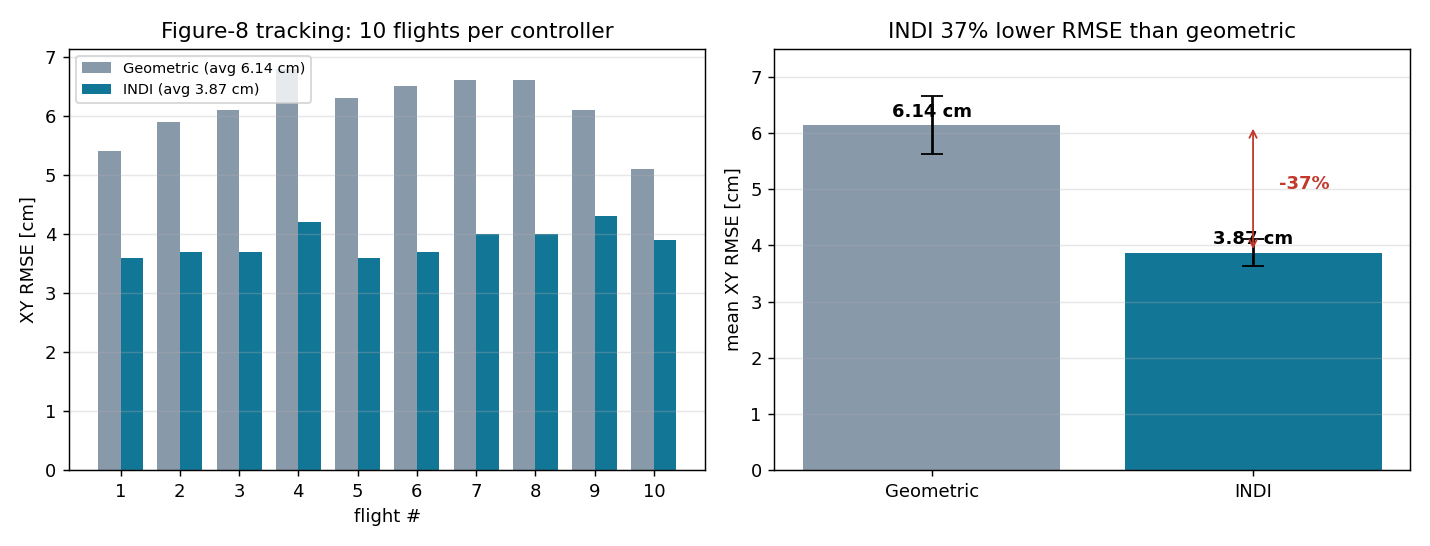
\includegraphics[width=0.72\linewidth]{flying_drone_stack/results/indi_commissioning/geo_vs_indi.png}
  \caption{Standard CF2.1: geometric vs.\ full-INDI, 10 flights each, figure-8 at $k_t=0.05$.}
  \label{fig:geo-vs-indi}
\end{figure}

\begin{figure}[h]
  \centering
  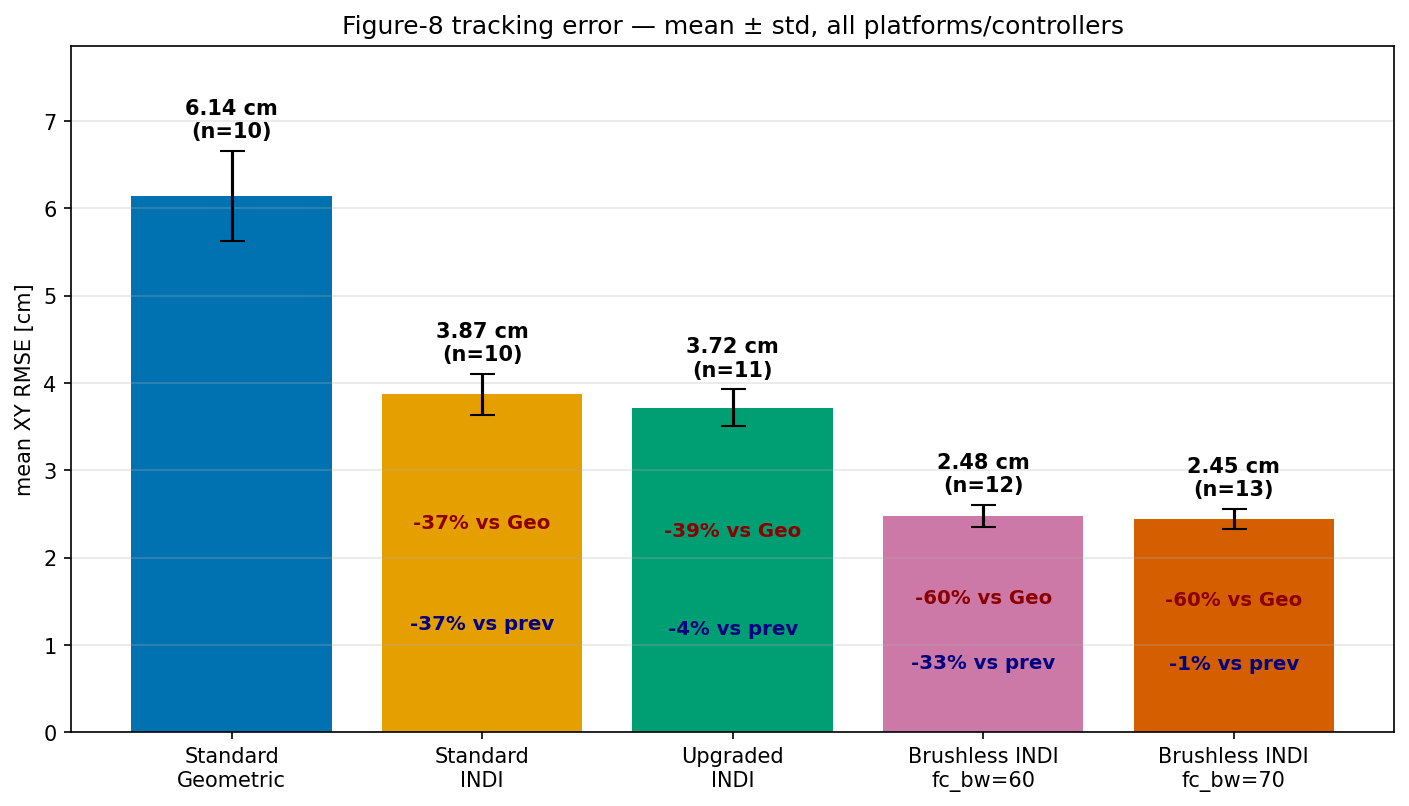
\includegraphics[width=0.72\linewidth]{flying_drone_stack/docs/5way_mean_comparison.png}
  \caption{Five-way headline comparison: mean XY RMSE across all platform/controller
    configurations, figure-8 at $k_t=0.05$.}
  \label{fig:5way}
\end{figure}

\begin{figure}[t]
  \centering
  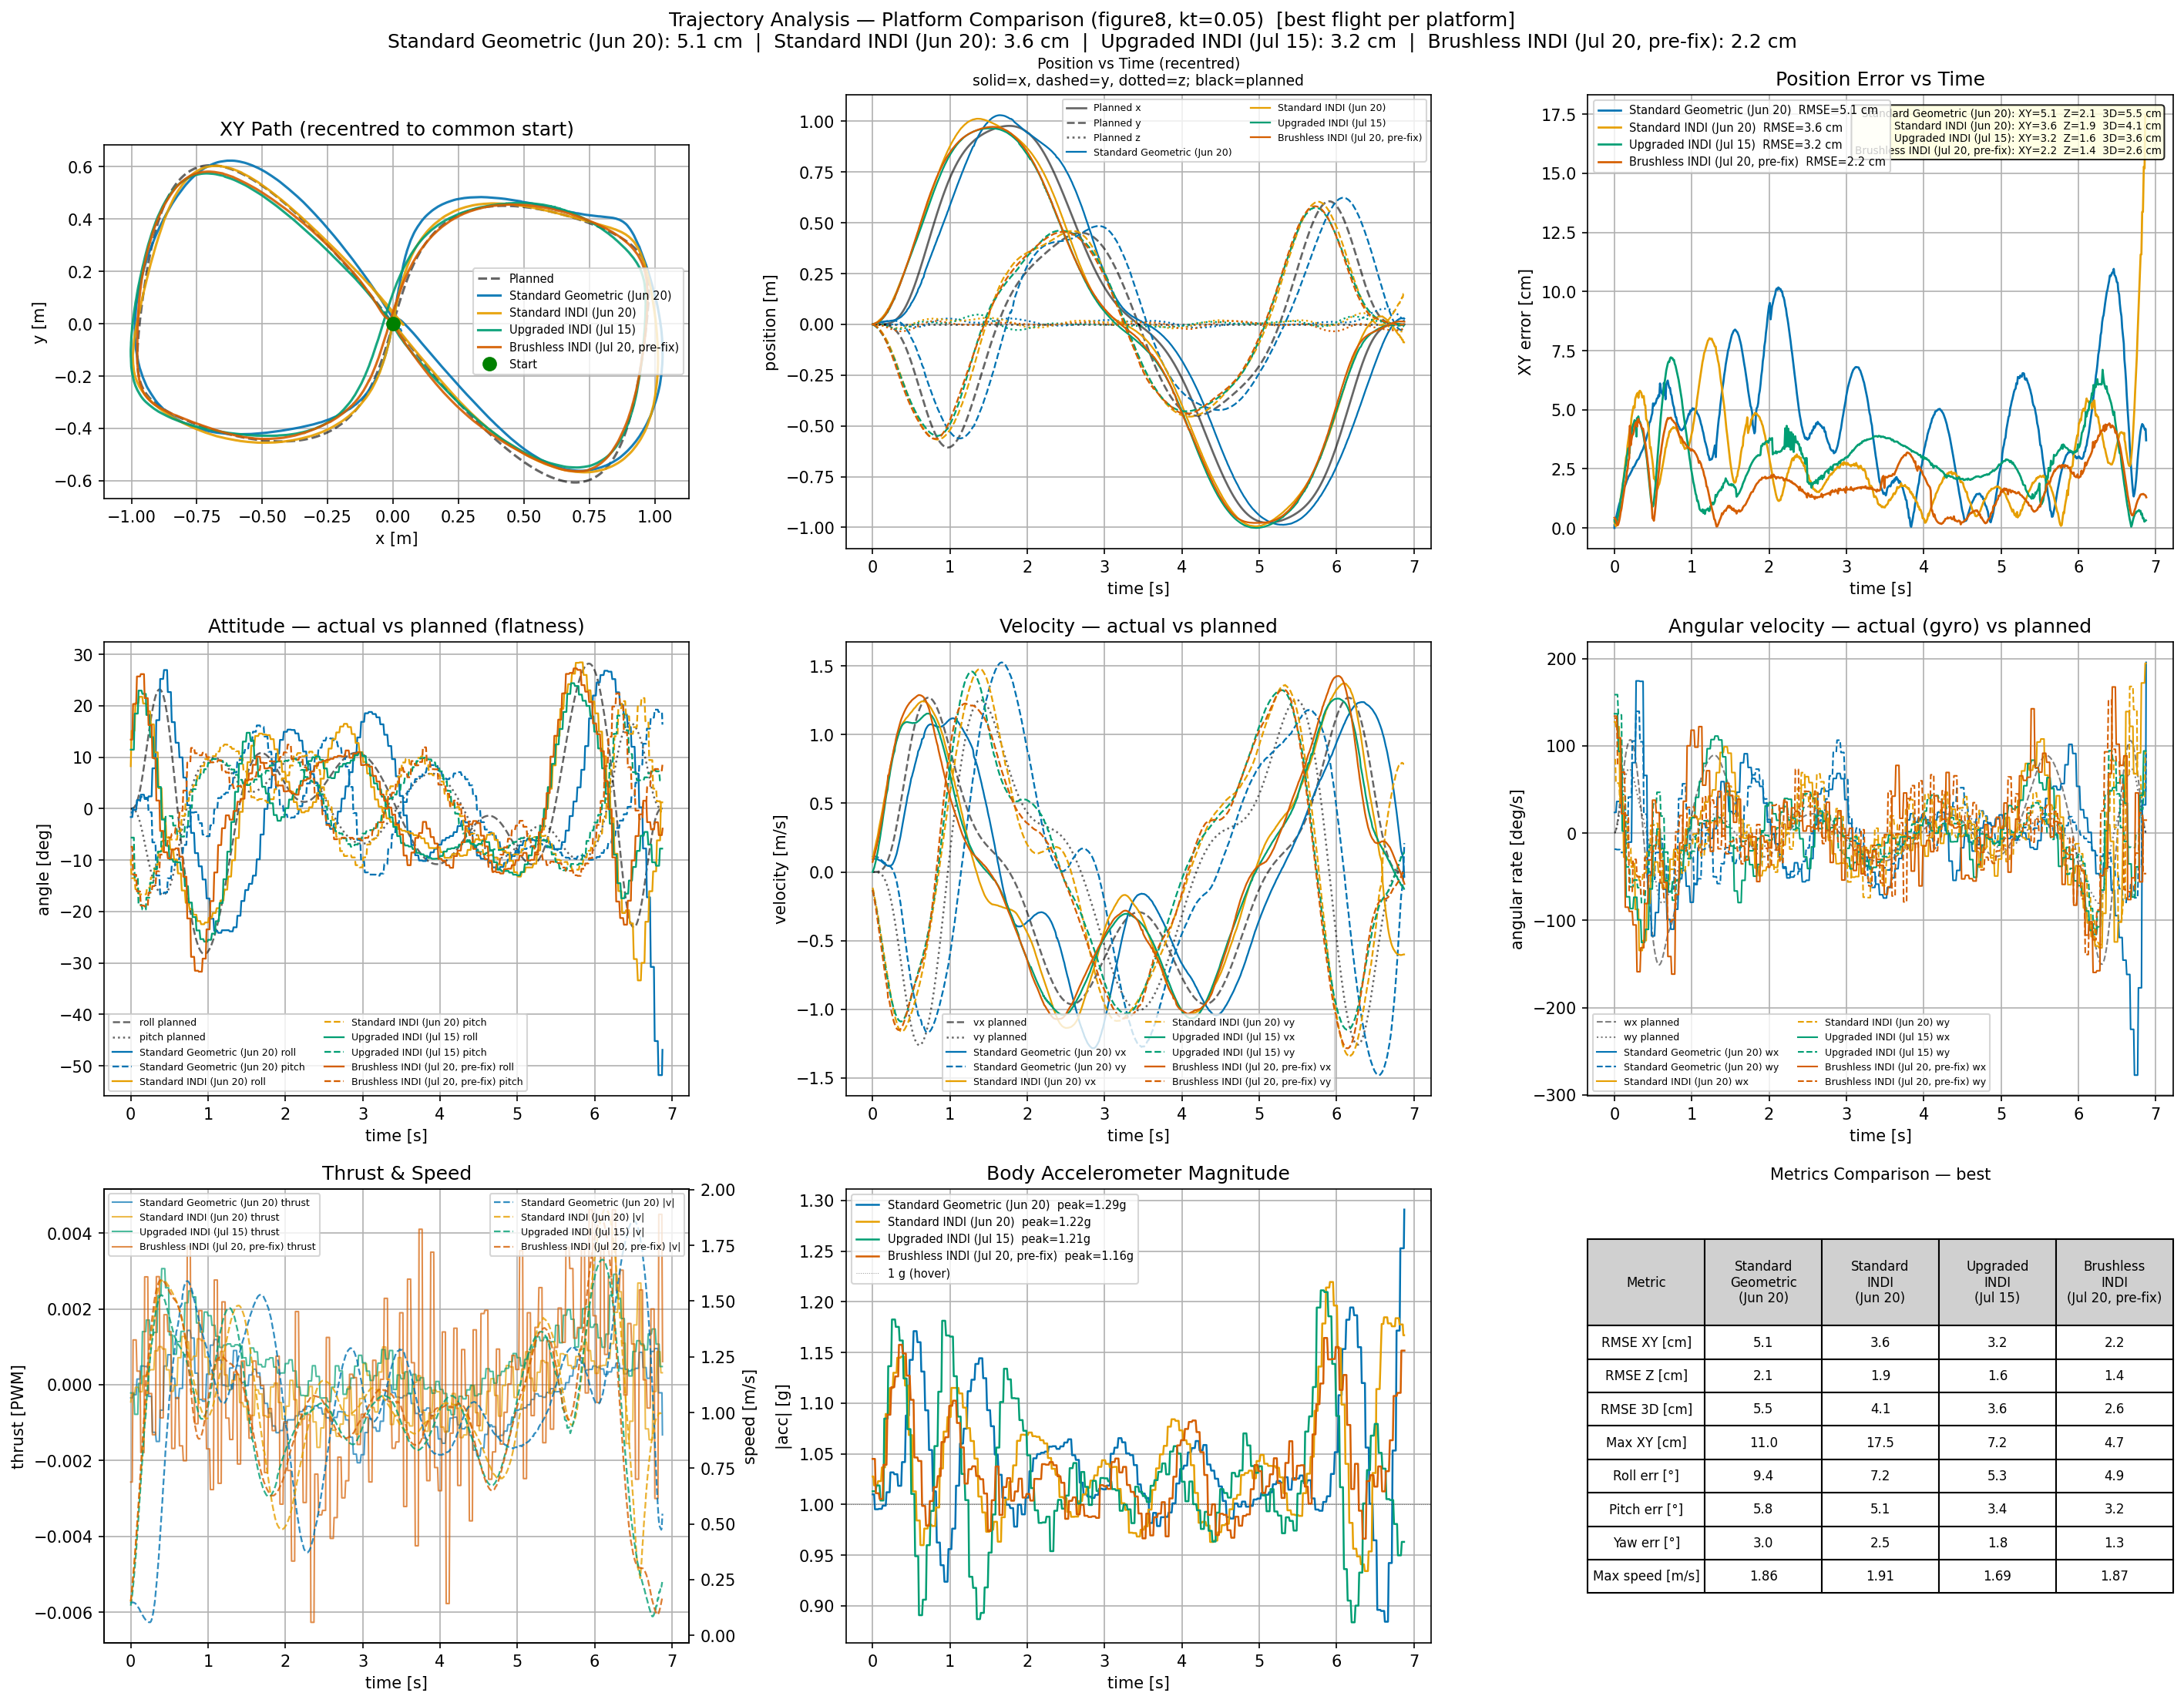
\includegraphics[width=0.72\linewidth]{flying_drone_stack/docs/platform_compare_best_analysis.png}
  \caption{Best flight, brushless platform, figure-8 at $k_t=0.05$: XY tracking overview.}
  \label{fig:best-analysis}
\end{figure}

\begin{figure}[t]
  \centering
  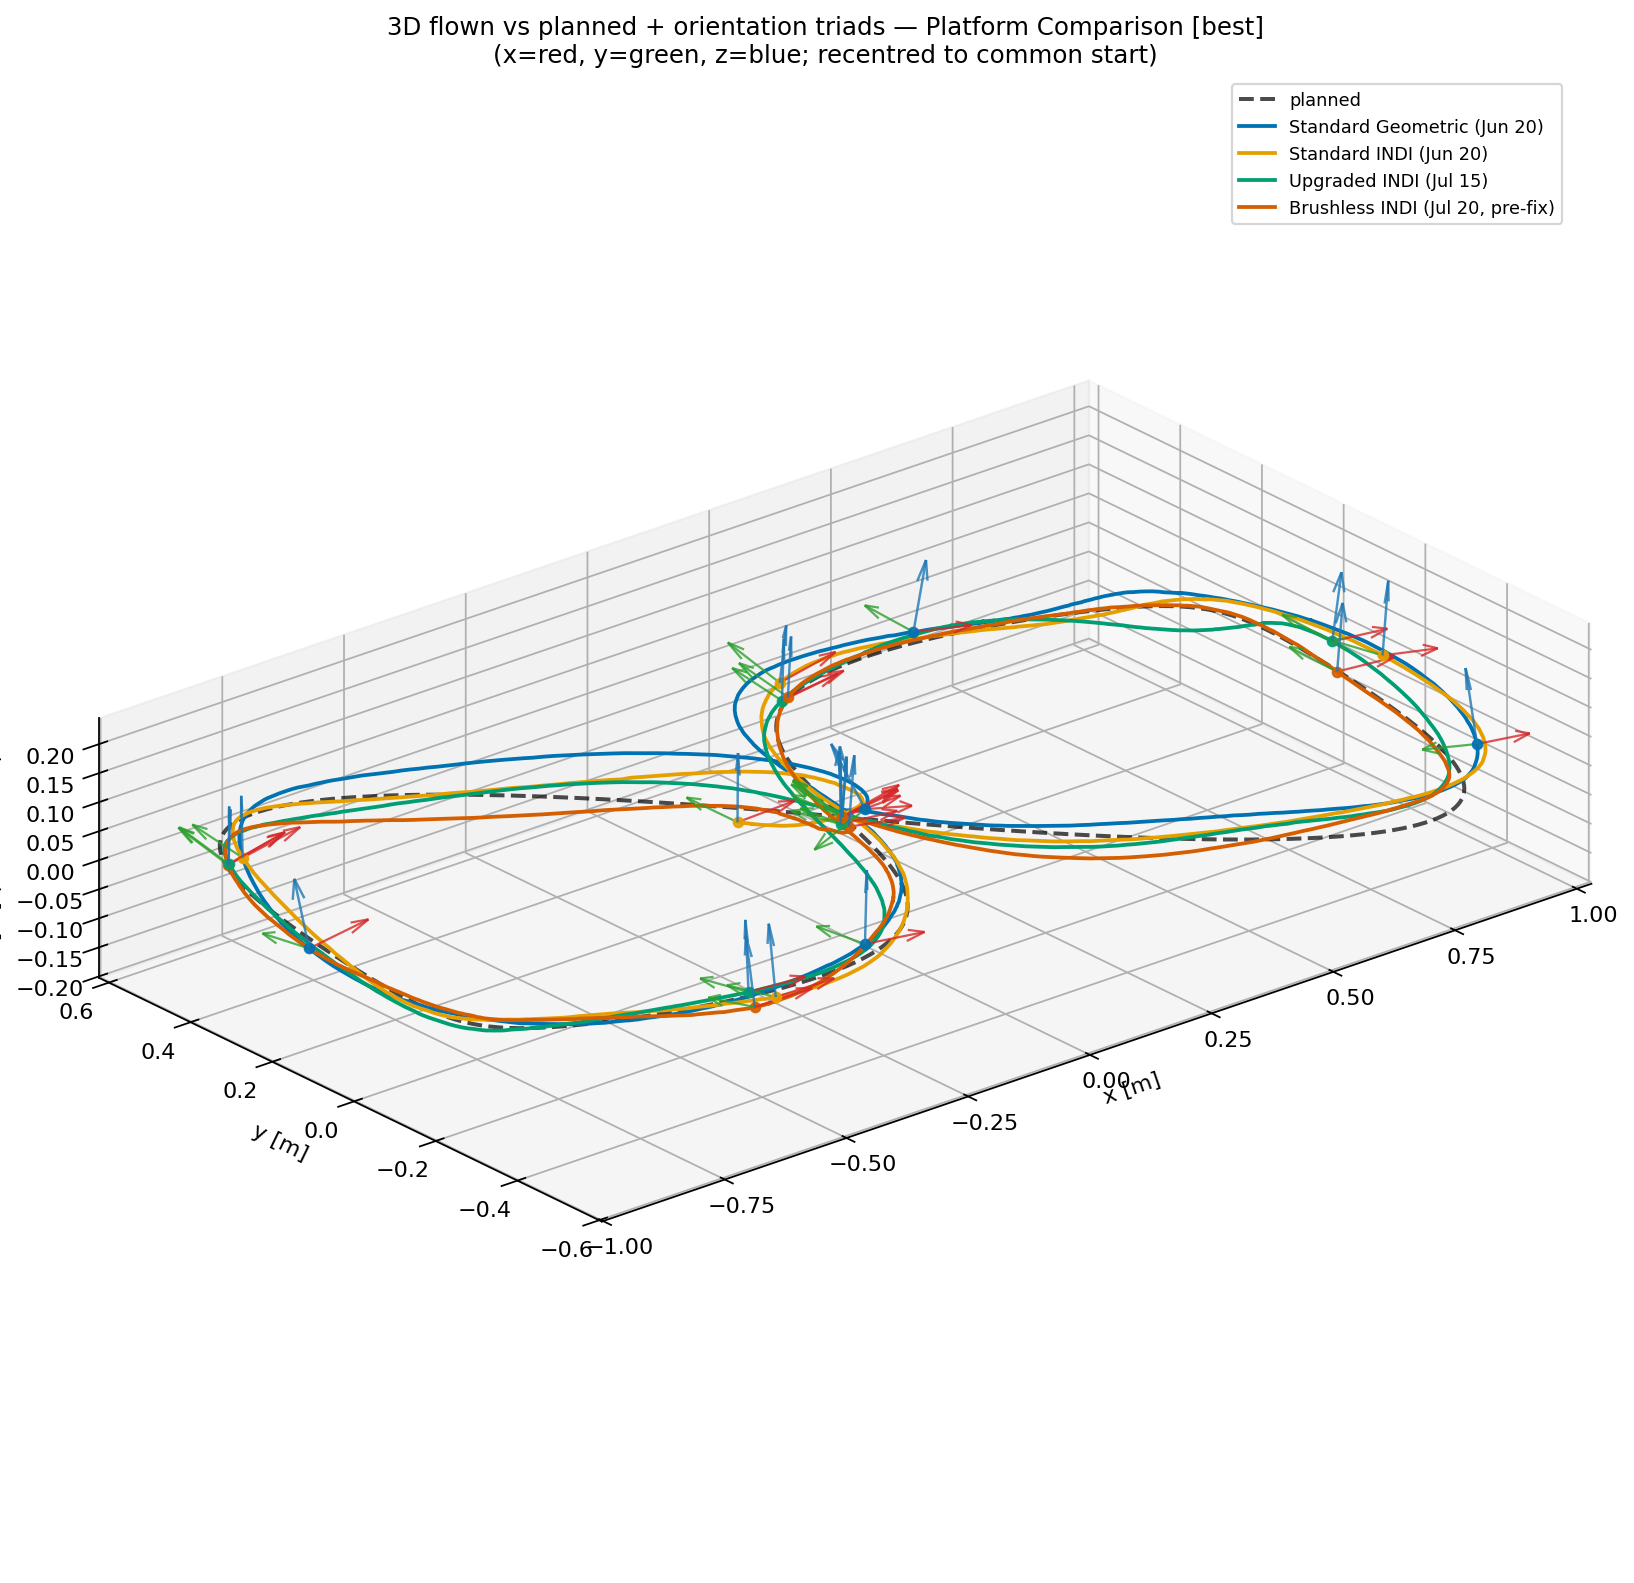
\includegraphics[width=0.72\linewidth]{flying_drone_stack/docs/platform_compare_best_3d_orientation.png}
  \caption{Best flight, brushless platform: 3D orientation.}
  \label{fig:best-3d}
\end{figure}

\begin{figure}[t]
  \centering
  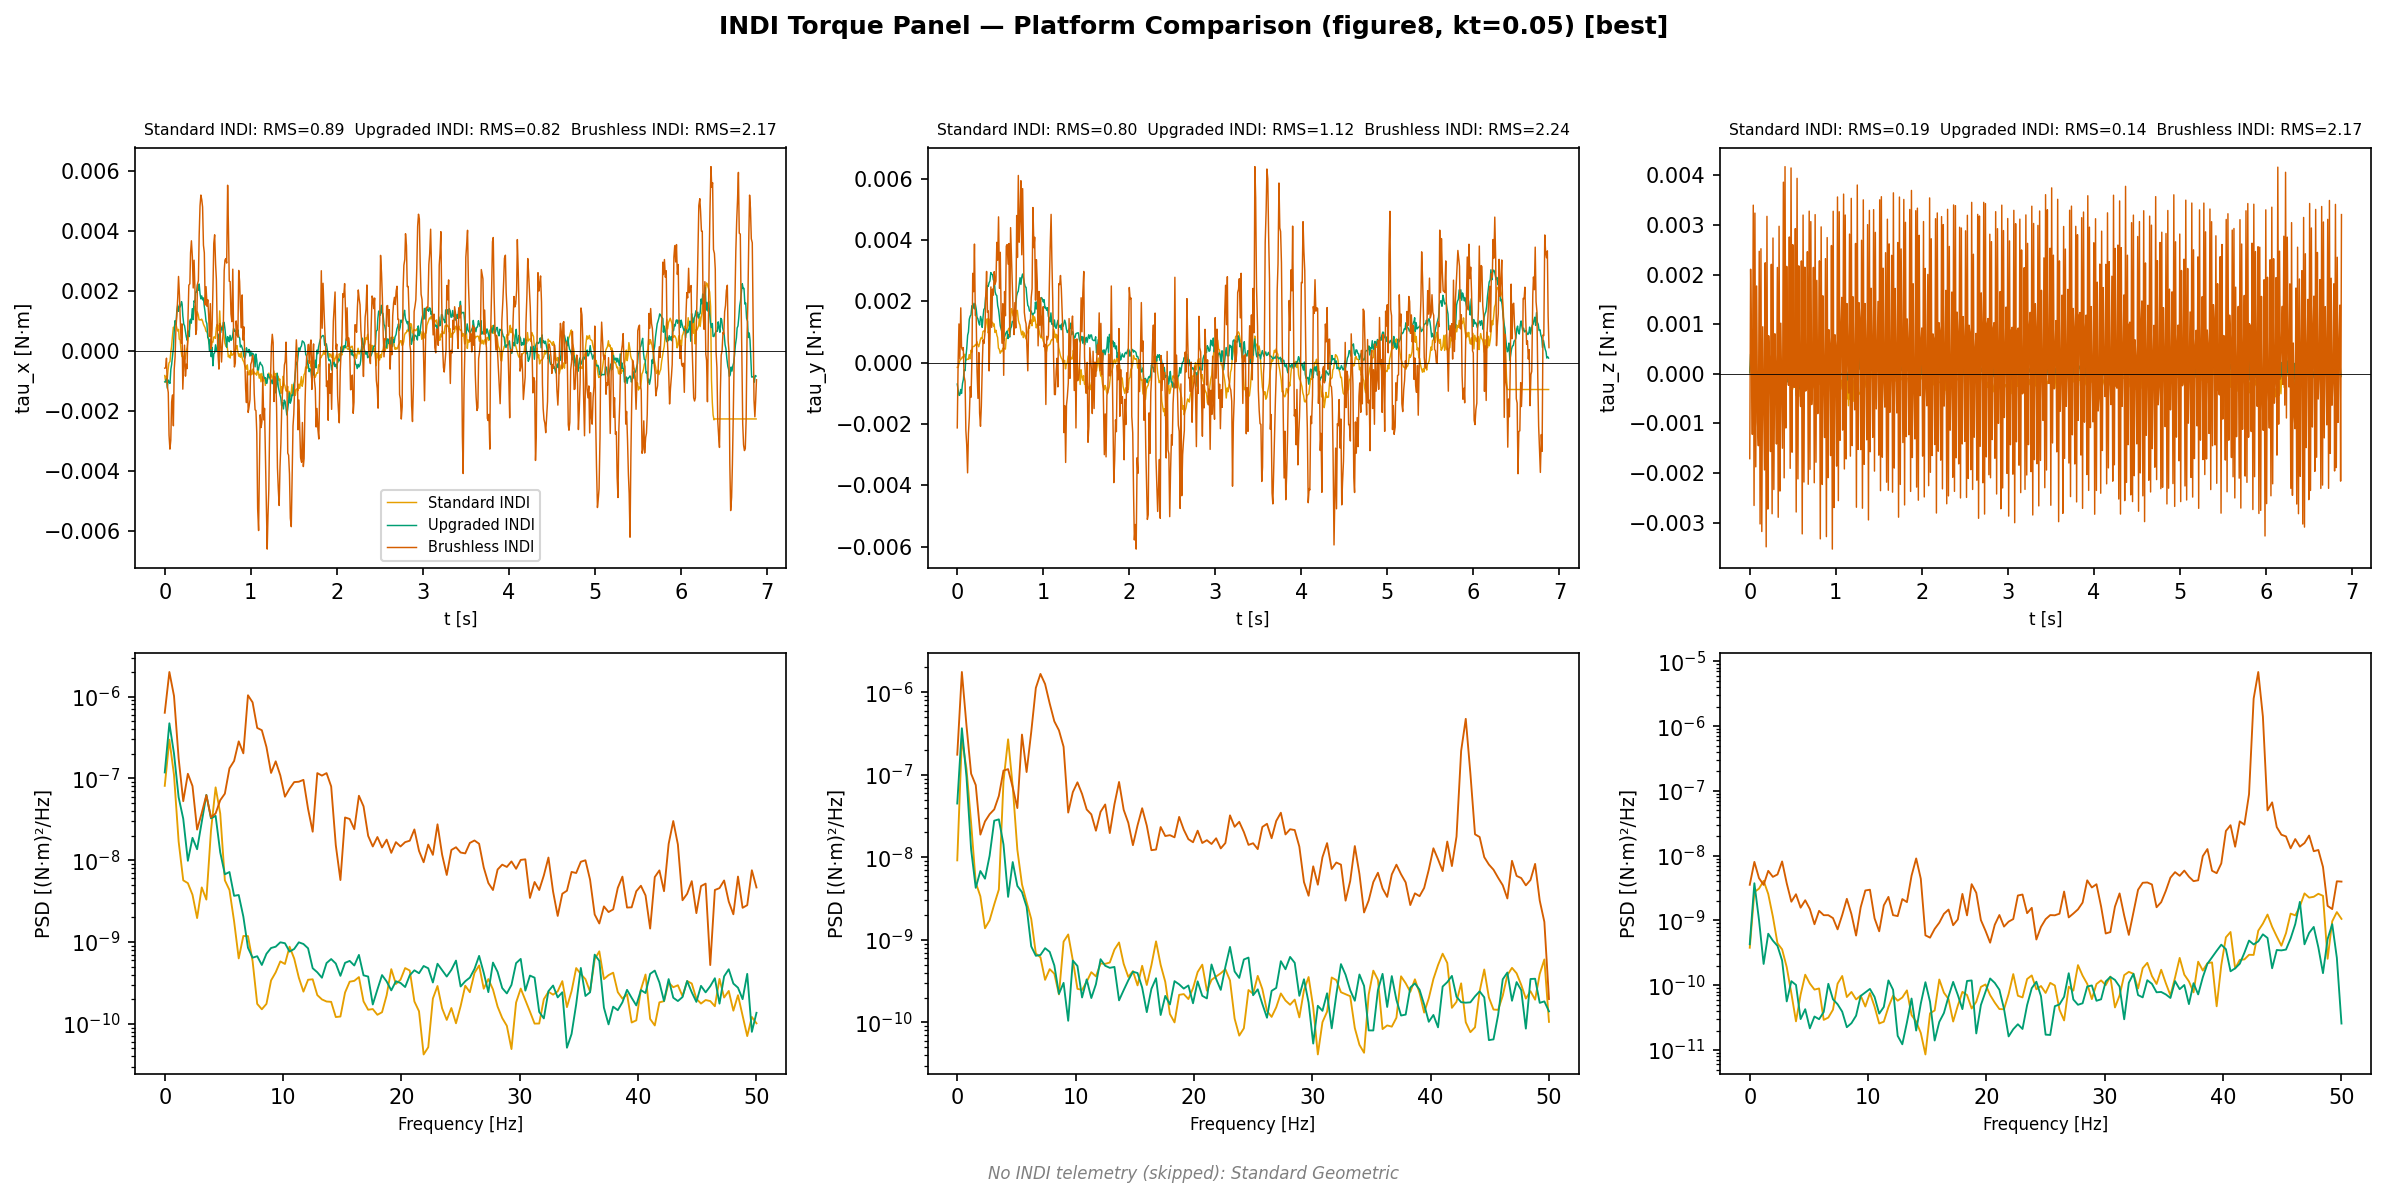
\includegraphics[width=0.72\linewidth]{flying_drone_stack/docs/platform_compare_best_indi_panel.png}
  \caption{Best flight, brushless platform: INDI torque/angular-acceleration panel.}
  \label{fig:best-indi}
\end{figure}

\begin{figure}[t]
  \centering
  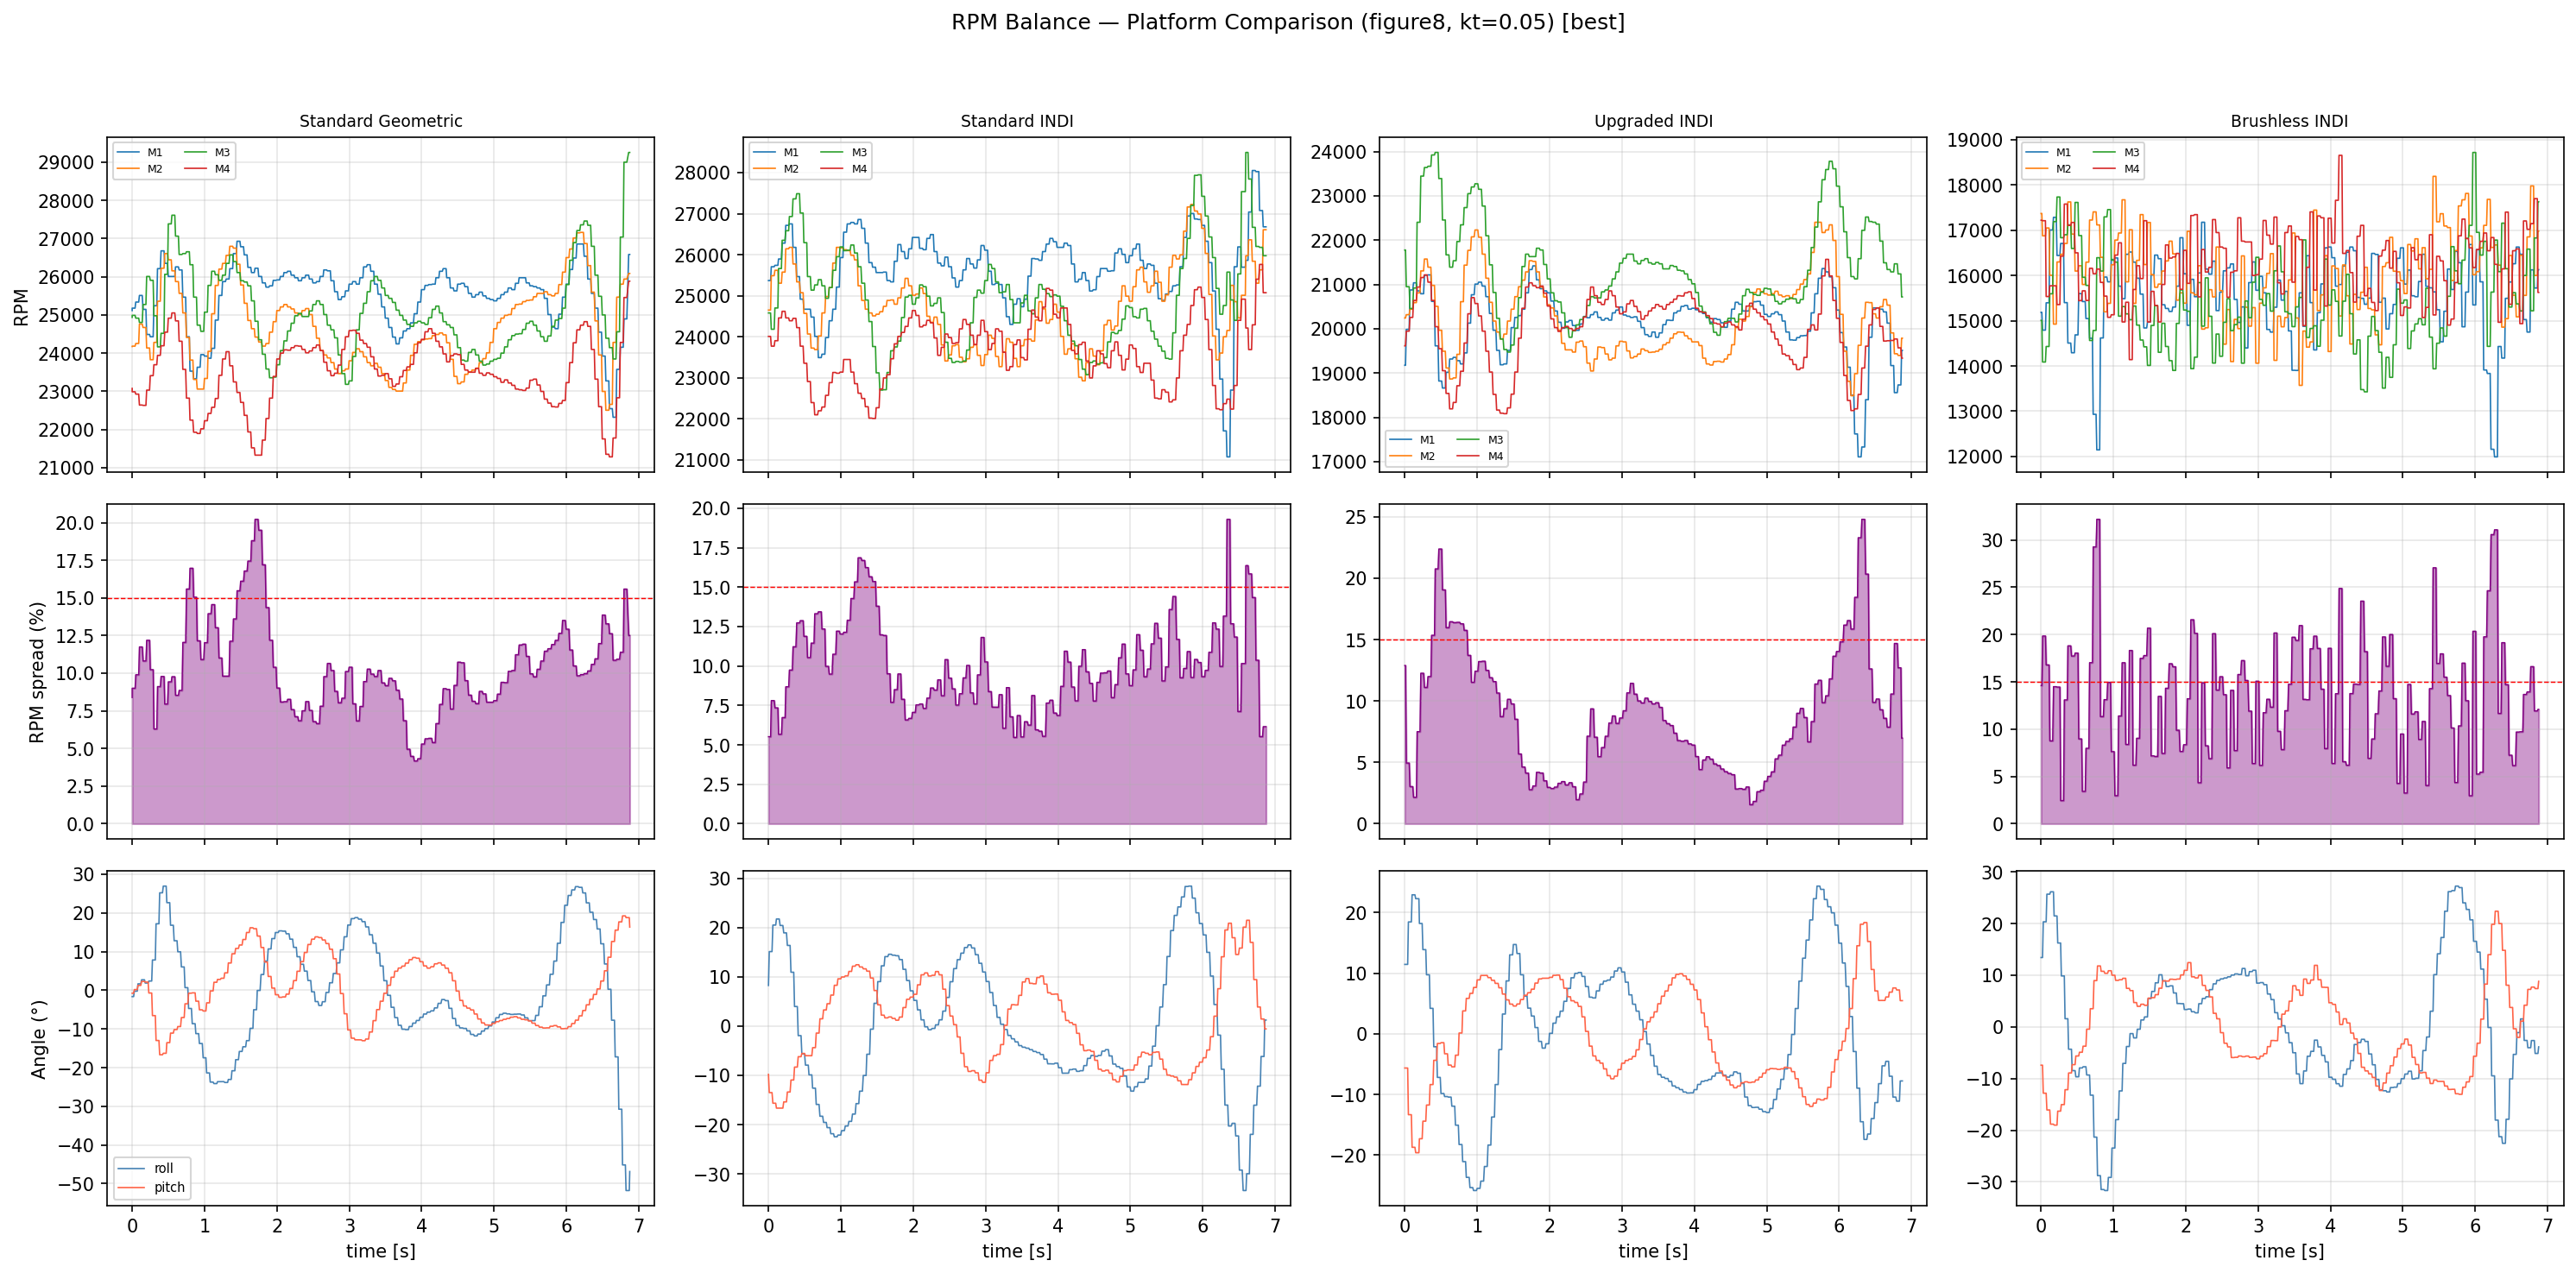
\includegraphics[width=0.72\linewidth]{flying_drone_stack/docs/platform_compare_best_rpm_balance.png}
  \caption{Best flight, brushless platform: per-motor RPM balance.}
  \label{fig:best-rpm}
\end{figure}

\begin{figure}[t]
  \centering
  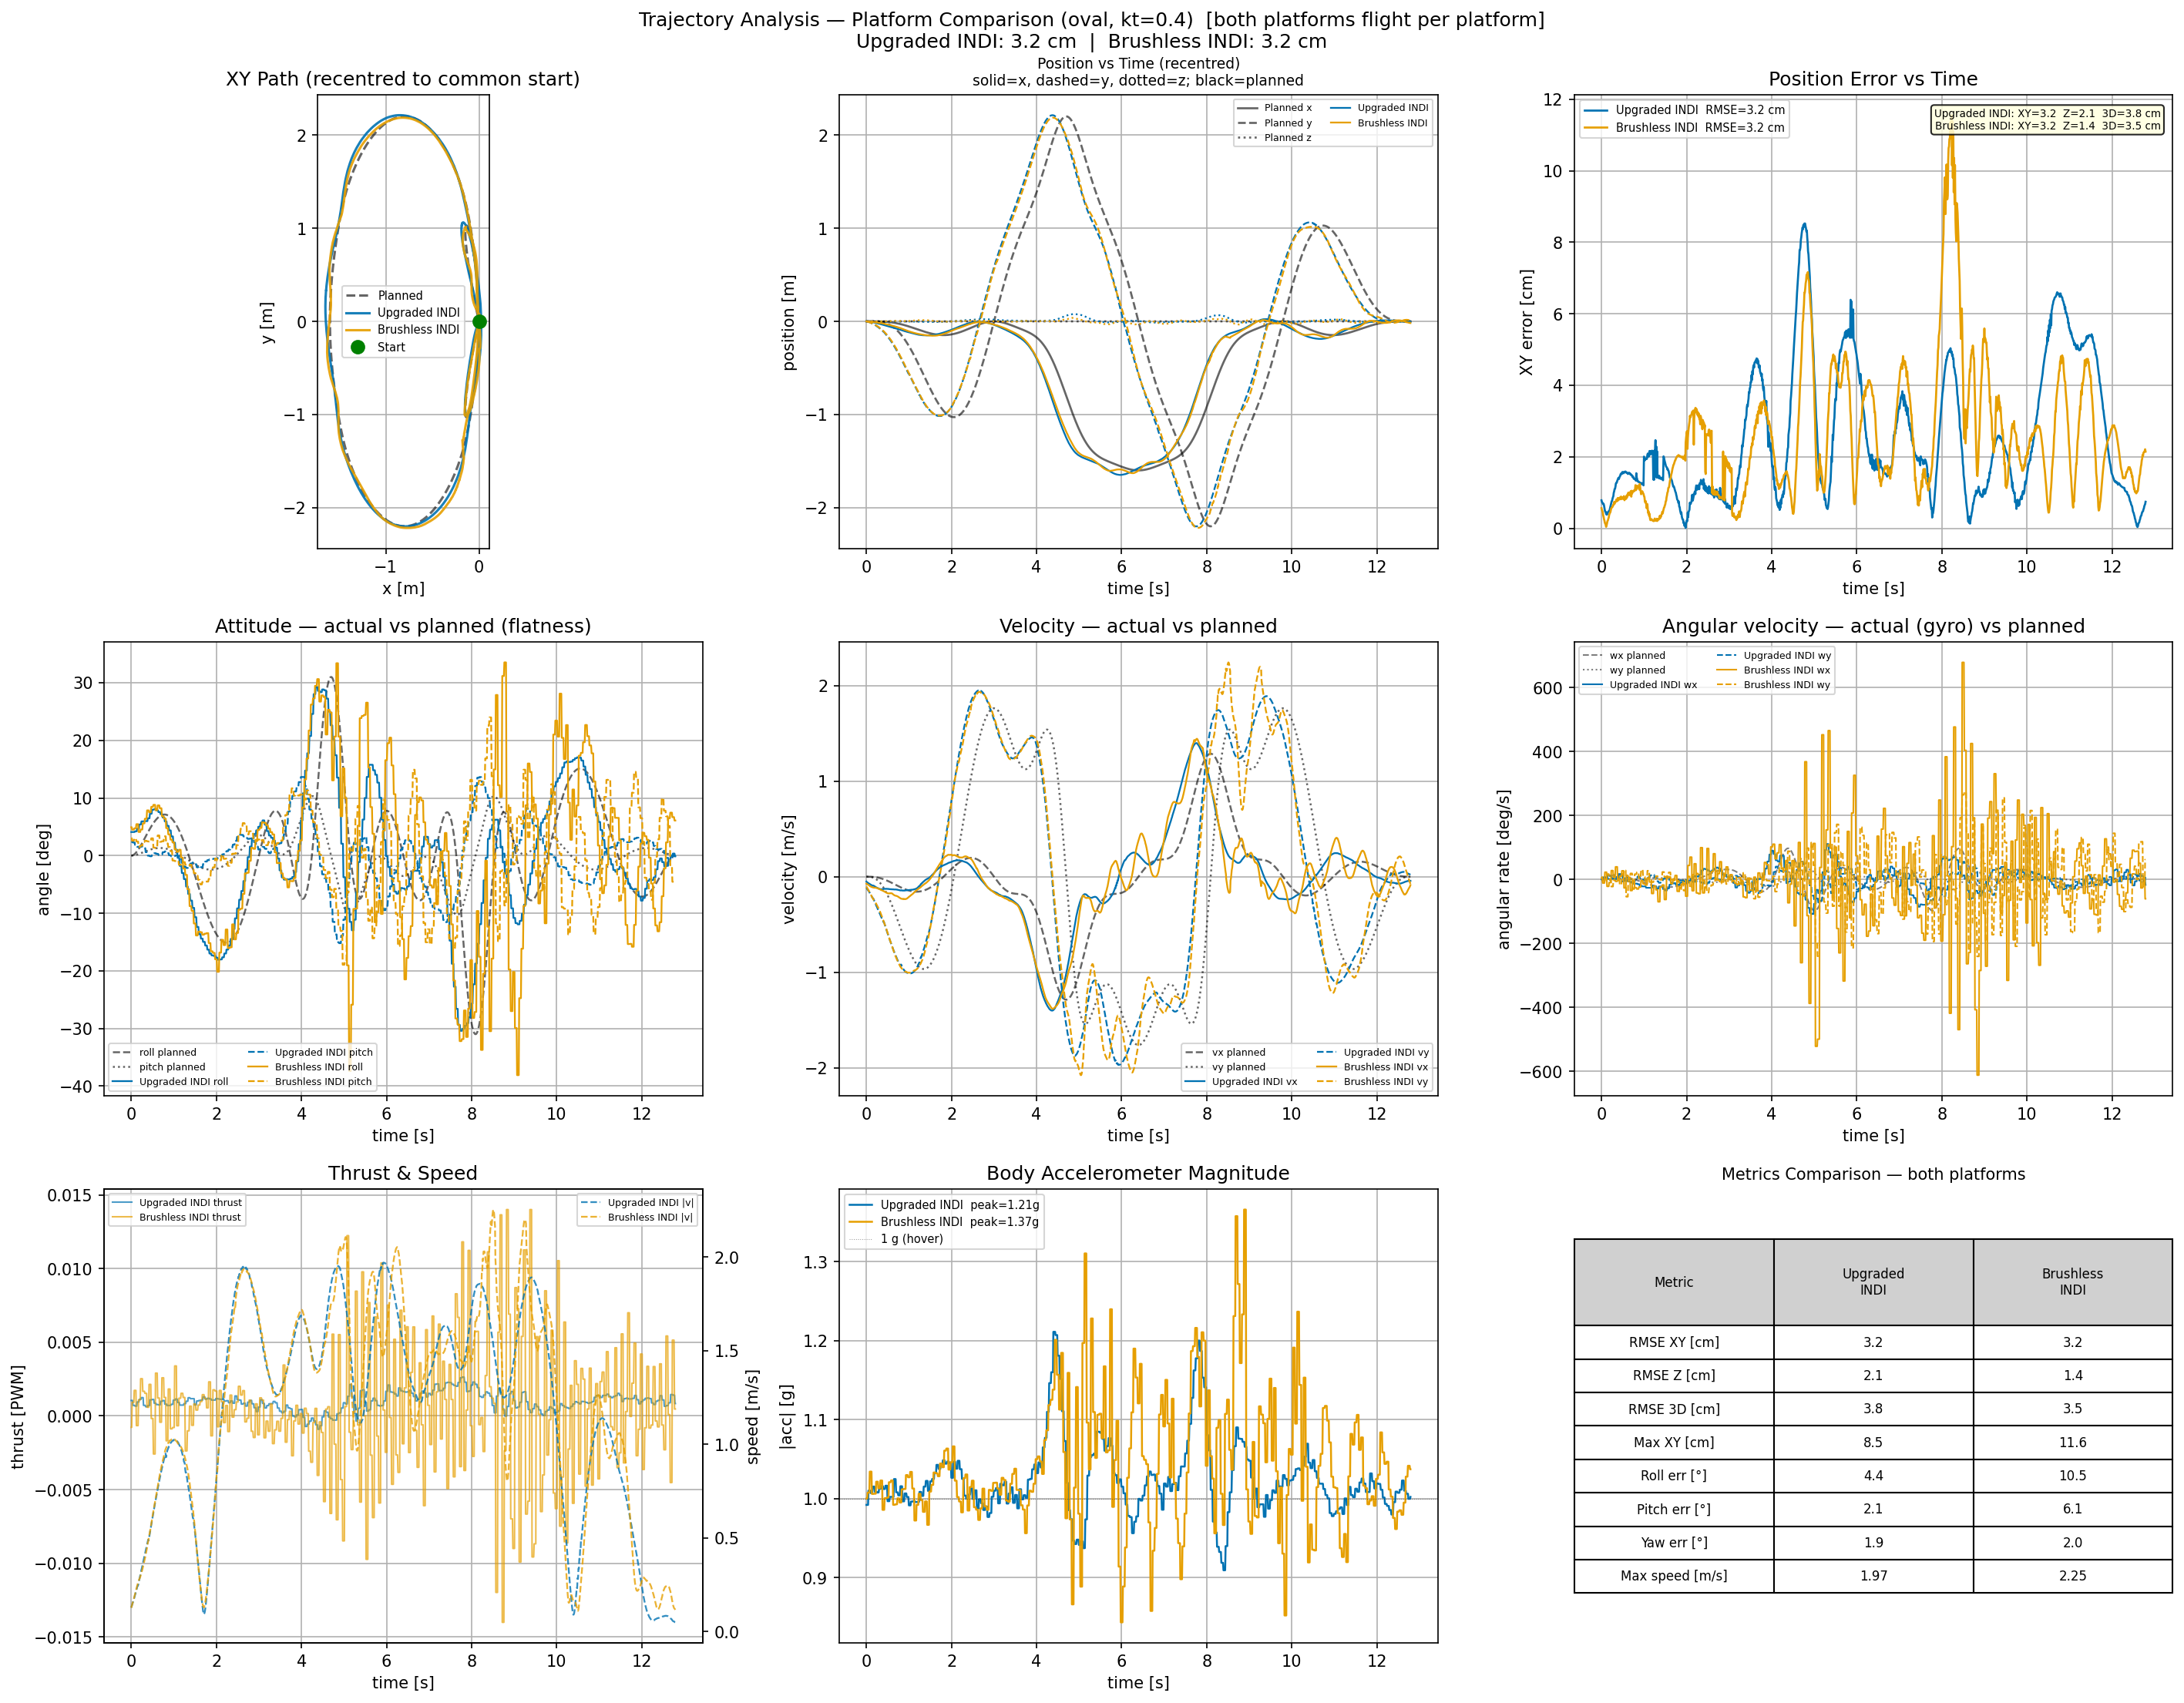
\includegraphics[width=0.72\linewidth]{Controls/logs/platform_compare_oval_kt0.4_analysis.png}
  \caption{Upgraded vs.\ brushless tracking overview, oval trajectory at $k_t=0.4$.}
  \label{fig:oval-kt04}
\end{figure}

\begin{figure}[t]
  \centering
  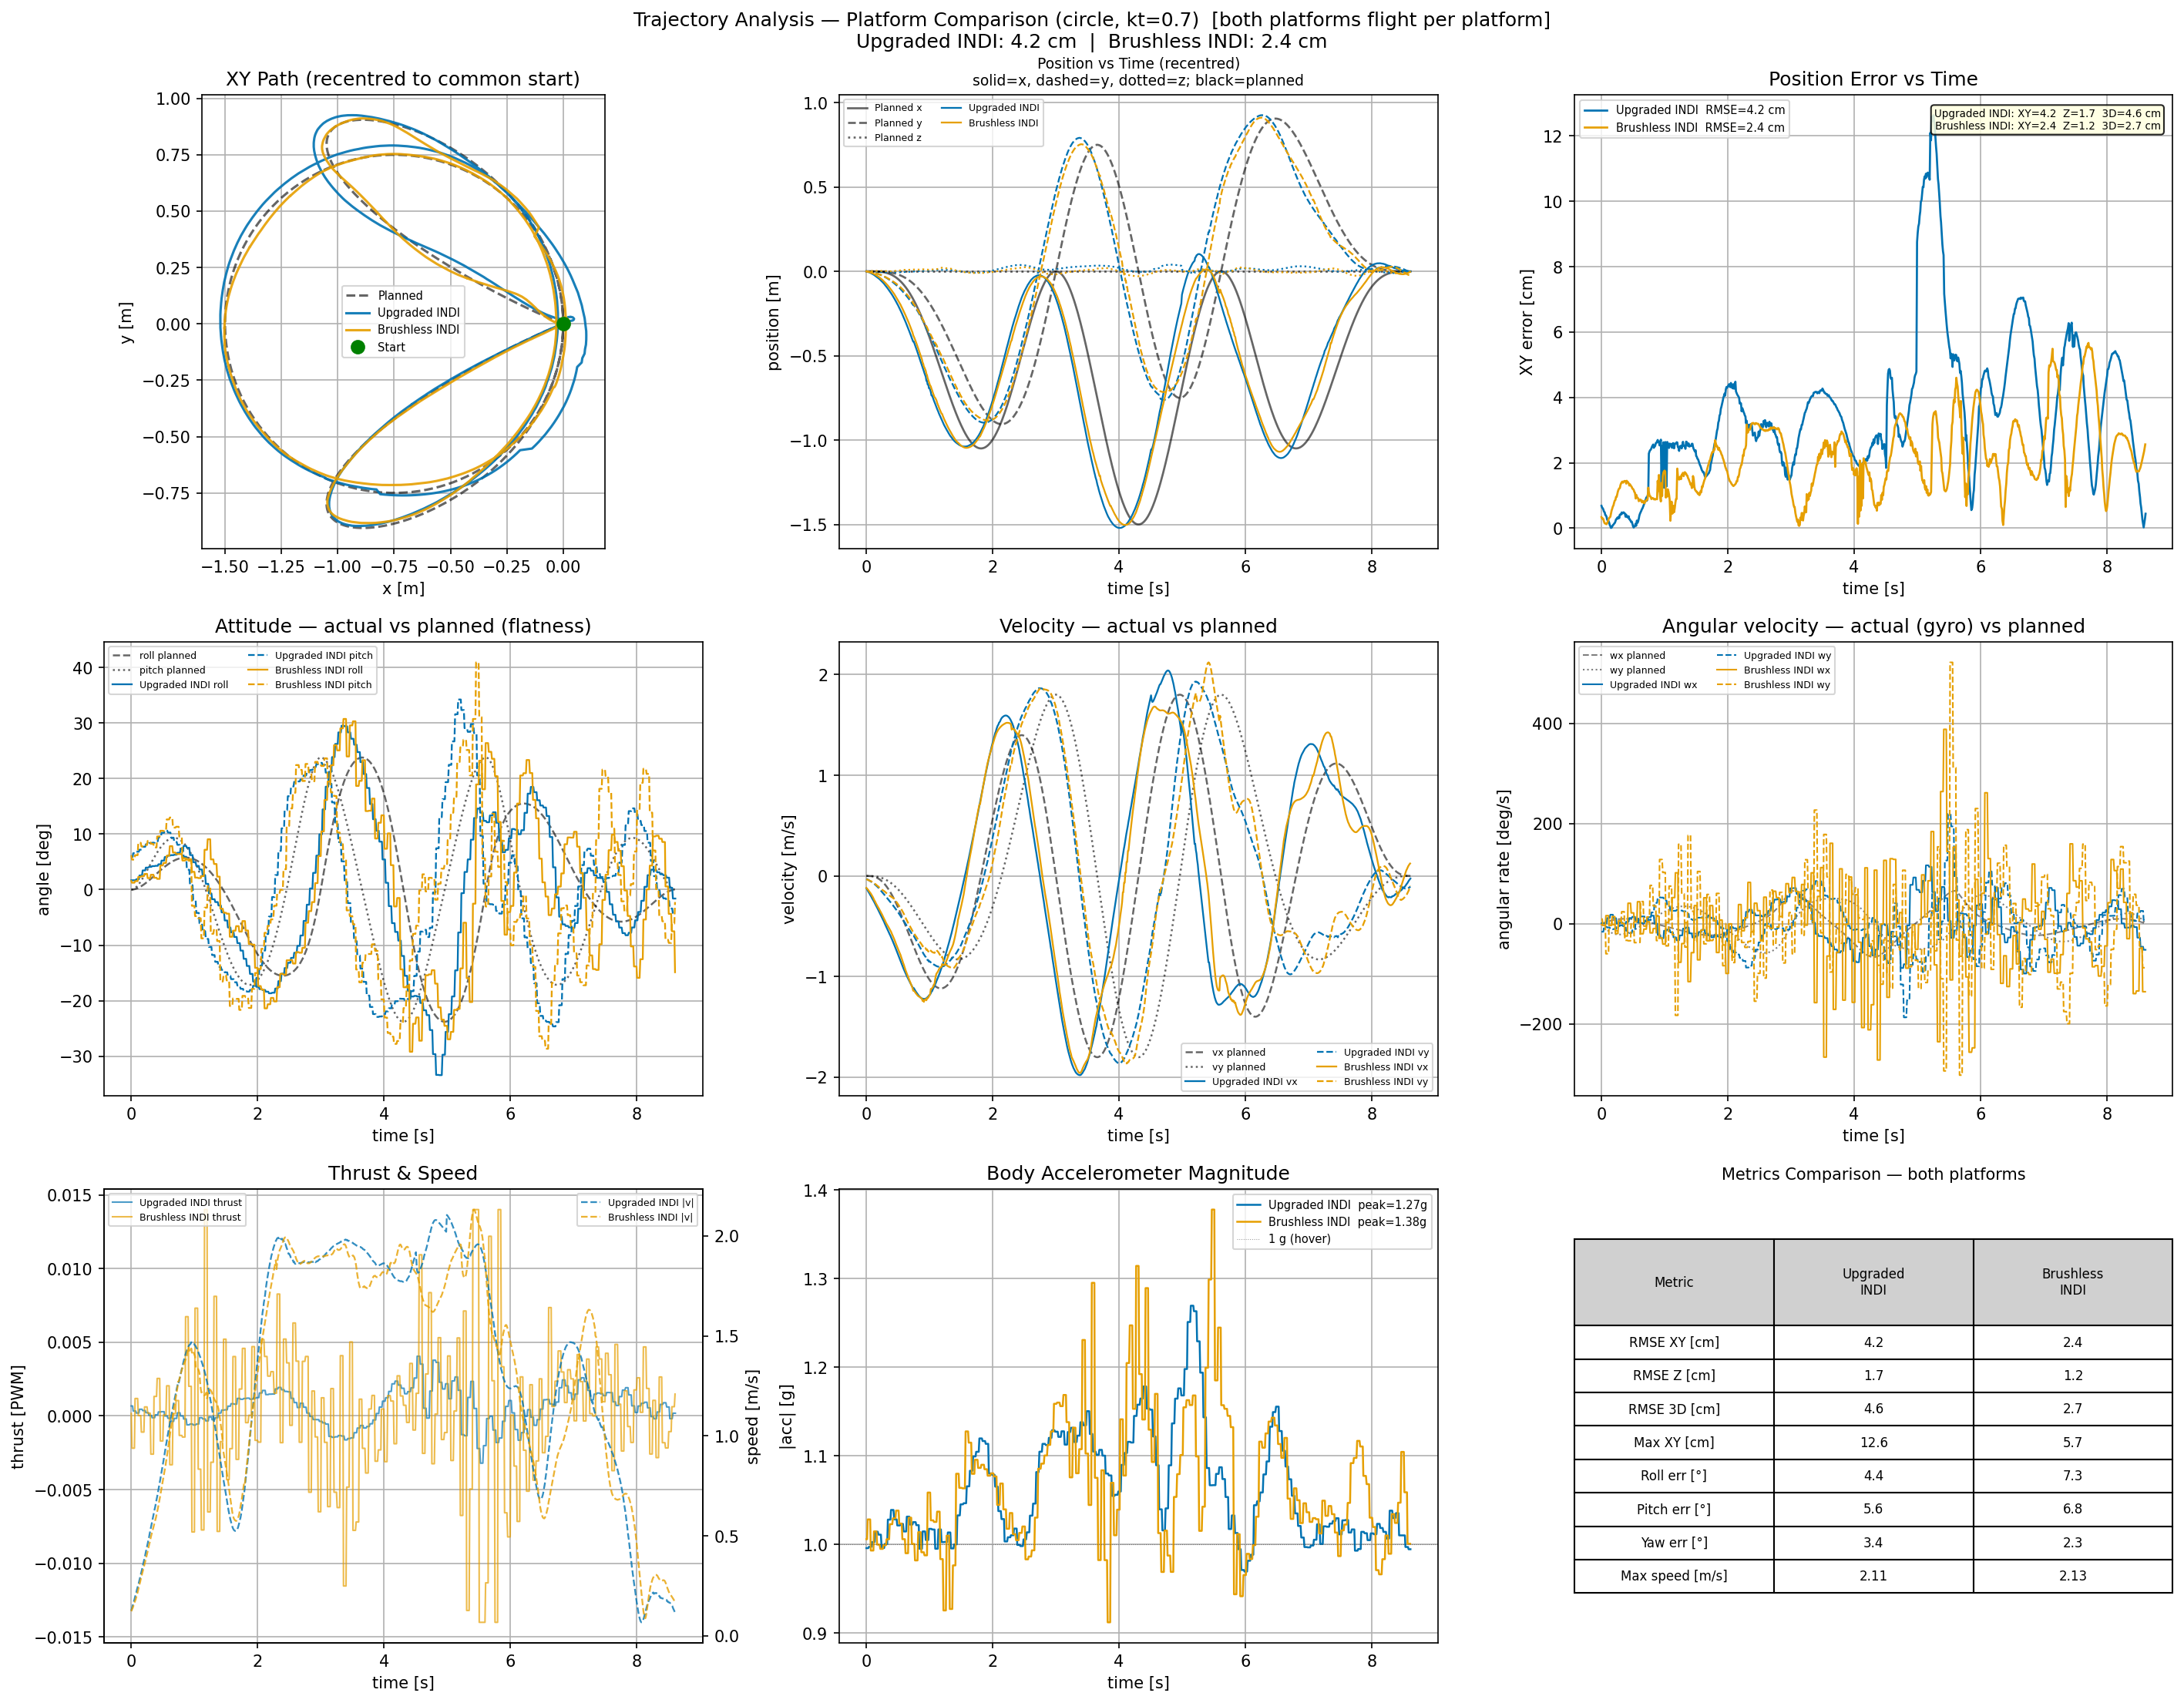
\includegraphics[width=0.72\linewidth]{Controls/logs/platform_compare_circle_kt0.7_analysis.png}
  \caption{Upgraded vs.\ brushless tracking overview, circle trajectory at $k_t=0.7$.}
  \label{fig:circle-kt07}
\end{figure}

\begin{figure}[t]
  \centering
  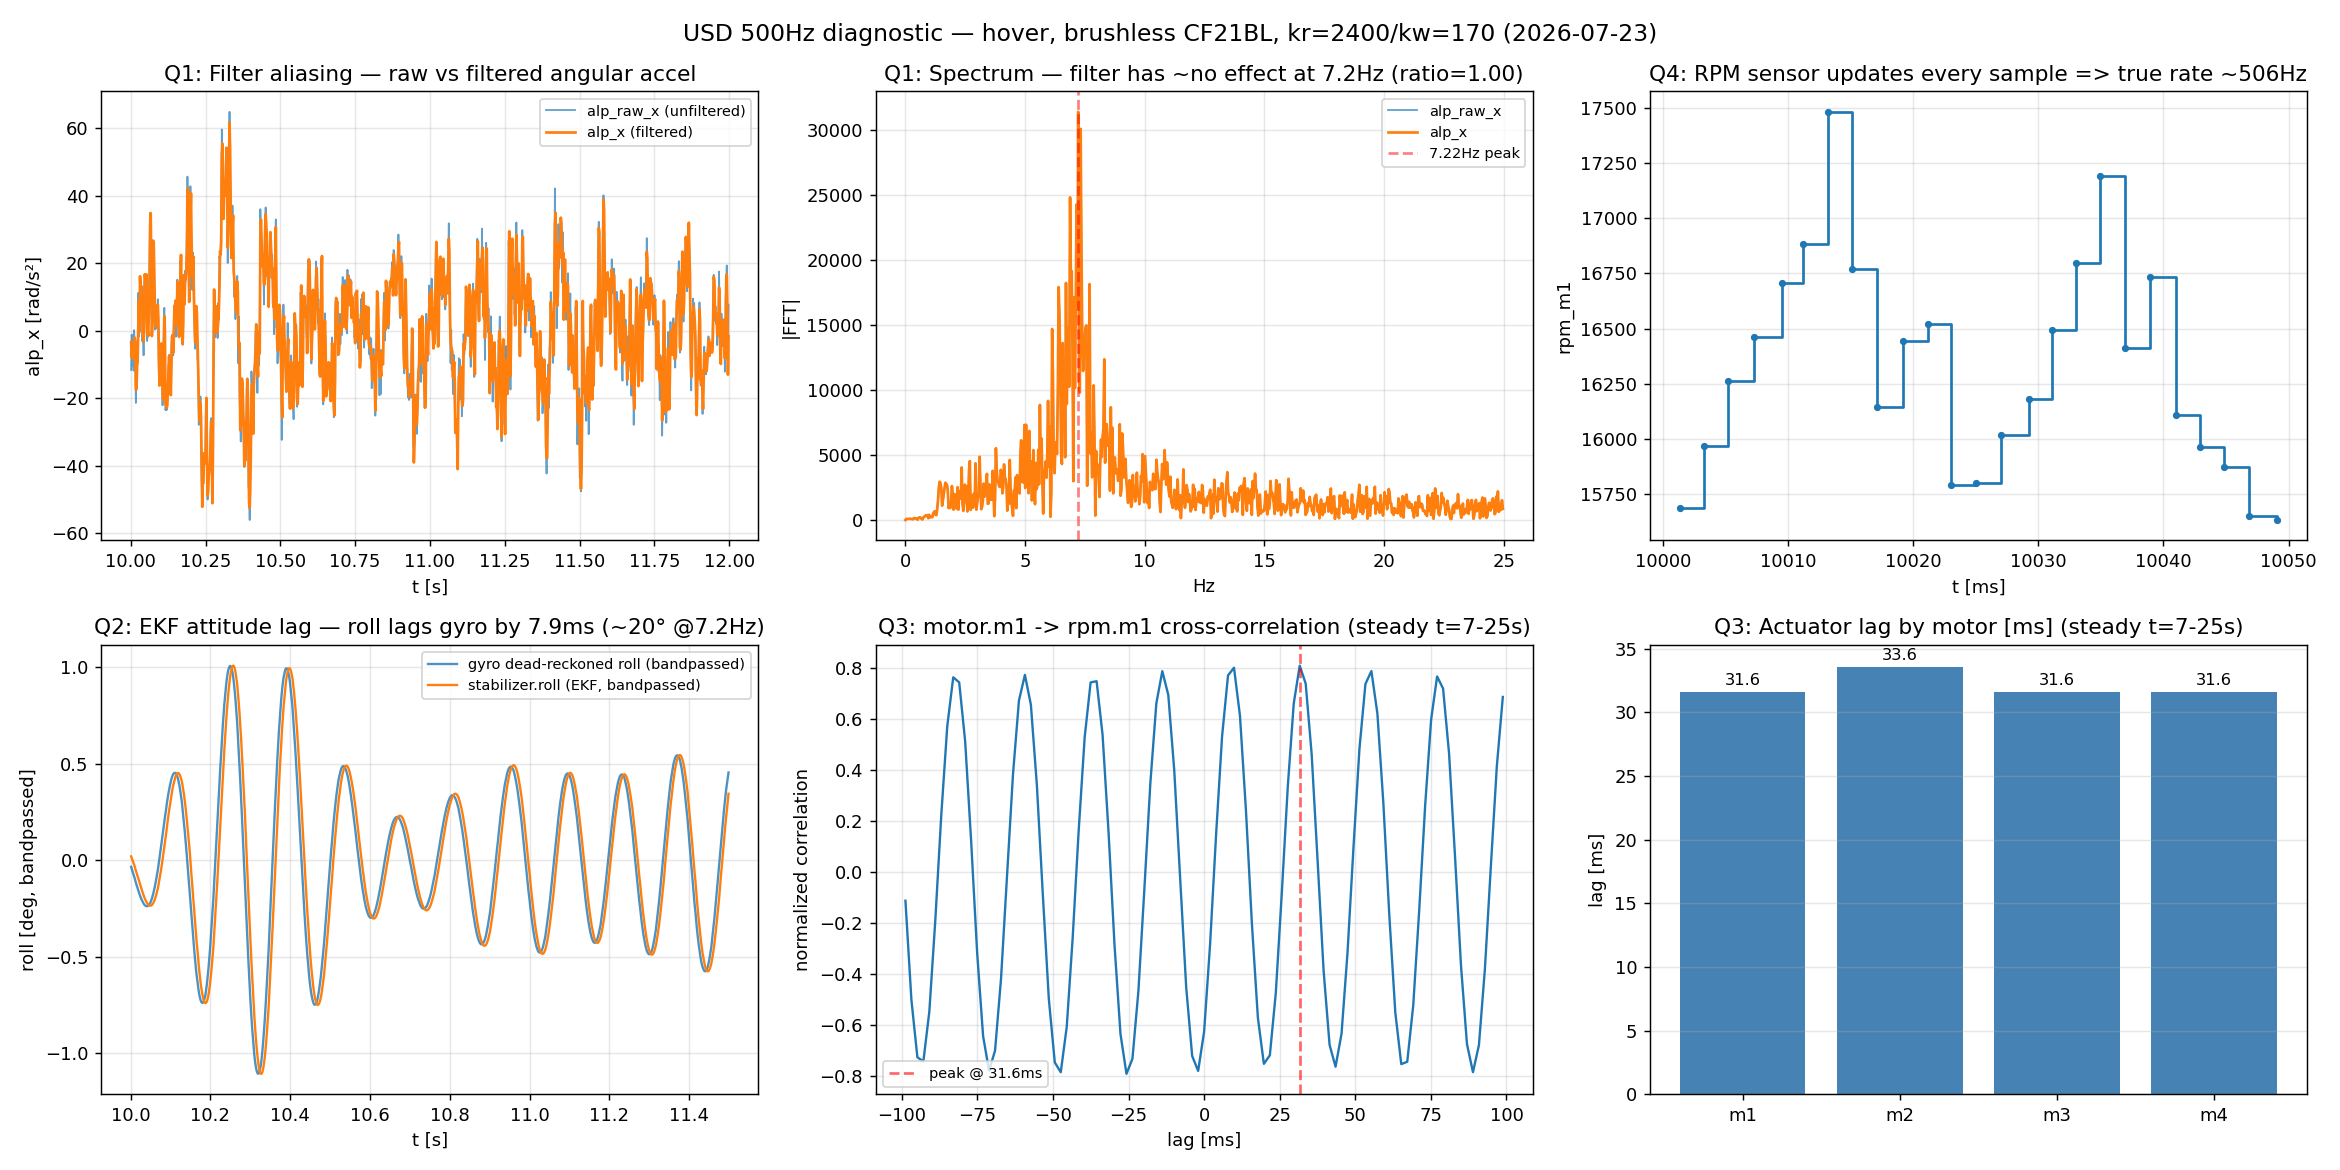
\includegraphics[width=0.72\linewidth]{flying_drone_stack/docs/usd_hover_2026-07-23_shake_diagnostic.png}
  \caption{500\,Hz SD-card diagnostic at hover, brushless platform: the $\approx$7.22\,Hz
    resonance quantified.}
  \label{fig:shake-hover}
\end{figure}

\begin{figure}[t]
  \centering
  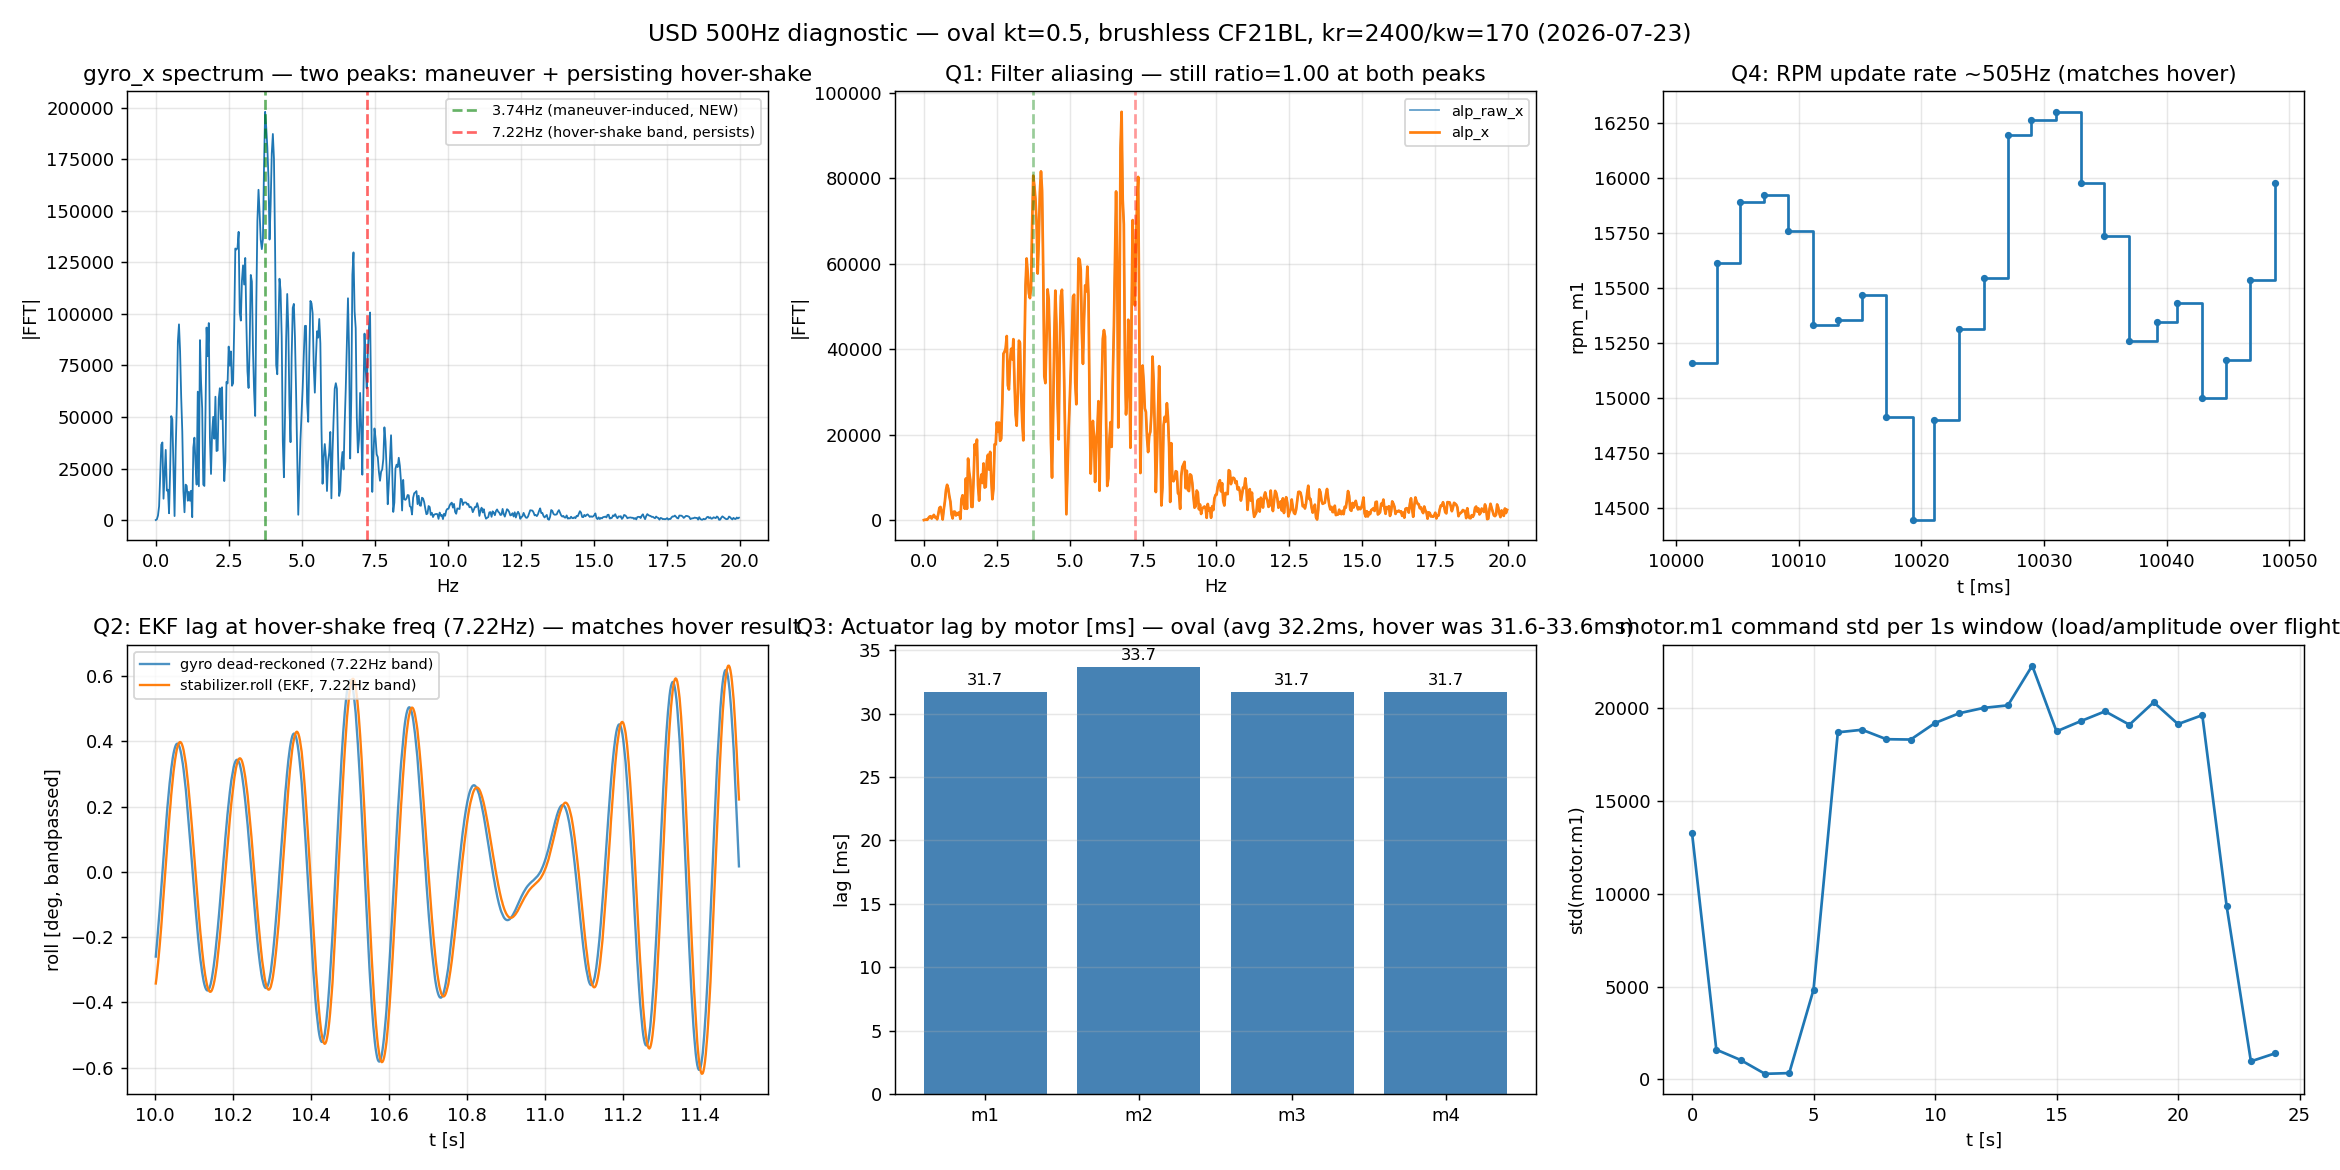
\includegraphics[width=0.72\linewidth]{flying_drone_stack/docs/usd_oval_2026-07-23_shake_diagnostic.png}
  \caption{500\,Hz SD-card diagnostic under an oval maneuver, brushless platform: the resonance
    persists unchanged under real maneuvering load.}
  \label{fig:shake-oval}
\end{figure}

\clearpage
%======================================================================
\section{Full $k_t$-Sweep Data}
\label{sec:appendix-ktsweep}
%======================================================================

Full per-$k_t$ data underlying the oval and circle summaries in
Section~\ref{sec:extended-sweeps}, both platforms. ``Crash'' entries are excluded from the
RMSE/error/speed columns for that $k_t$.

\begin{table}[h]
\centering
\scriptsize
\renewcommand{\arraystretch}{1.15}
\begin{tabular}{@{}lcccccc@{}}
\toprule
& \multicolumn{2}{c}{XY / Z RMSE} & \multicolumn{2}{c}{Roll/Pitch/Yaw err} & \multicolumn{2}{c}{Max speed [m/s]} \\
\cmidrule(lr){2-3} \cmidrule(lr){4-5} \cmidrule(lr){6-7}
$k_t$ & Upgraded & Brushless & Upgraded & Brushless & Upgraded & Brushless \\
\midrule
0.05 & 2.1/0.8\,cm & 2.3/0.5\,cm & 1.7/1.3/0.8$^\circ$ & 2.2/2.9/0.9$^\circ$ & 1.10 & 1.22 \\
0.1  & 2.8/0.9\,cm & 1.3/0.7\,cm & 2.3/1.5/0.7$^\circ$ & 3.1/1.6/0.3$^\circ$ & 1.33 & 1.32 \\
0.2  & 2.9/1.3\,cm & 2.5/1.1\,cm & 3.3/1.5/1.0$^\circ$ & 2.6/1.3/0.4$^\circ$ & 1.61 & 1.51 \\
0.3  & 3.0/1.8\,cm & 2.8/1.0\,cm & 3.2/1.7/1.4$^\circ$ & 2.9/1.5/0.5$^\circ$ & 1.76 & 1.72 \\
0.4  & 3.2/2.1\,cm & 3.2/1.4\,cm & 4.4/2.1/1.9$^\circ$ & 10.5/6.1/2.0$^\circ$ & 1.97 & 2.25 \\
0.5  & \textbf{crash (5/5)} & 3.1/1.6\,cm & --- & 5.5/2.7/1.4$^\circ$ & --- & 2.20 \\
0.6  & \textbf{crash} & not flown & --- & --- & --- & --- \\
0.7  & not flown & \textbf{crash} & --- & --- & --- & --- \\
\bottomrule
\end{tabular}
\caption{Oval $k_t$ sweep, both platforms.}
\label{tab:oval-ktsweep}
\end{table}

\begin{table}[h]
\centering
\scriptsize
\renewcommand{\arraystretch}{1.1}
\begin{tabular}{@{}lcccccc@{}}
\toprule
& \multicolumn{2}{c}{XY / Z RMSE} & \multicolumn{2}{c}{Roll/Pitch/Yaw err} & \multicolumn{2}{c}{Max speed [m/s]} \\
\cmidrule(lr){2-3} \cmidrule(lr){4-5} \cmidrule(lr){6-7}
$k_t$ & Upgraded & Brushless & Upgraded & Brushless & Upgraded & Brushless \\
\midrule
0.05 & 1.7/0.8\,cm & 1.9/0.6\,cm & 2.1/1.8/0.8$^\circ$ & 1.9/1.4/0.6$^\circ$ & 1.03 & 1.21 \\
0.1  & 1.9/1.3\,cm & 1.7/0.6\,cm & 1.9/1.8/1.1$^\circ$ & 4.2/3.9/0.7$^\circ$ & 1.15 & 1.50 \\
0.2  & 2.3/1.2\,cm & 6.1/1.8\,cm & 2.2/1.8/1.4$^\circ$ & 14.5/13.2/3.6$^\circ$ & 1.35 & 1.71 \\
0.3  & 2.2/1.5\,cm & 1.4/0.8\,cm & 2.3/2.1/1.9$^\circ$ & 3.1/2.7/0.6$^\circ$ & 1.53 & 1.75 \\
0.4  & 2.7/1.8\,cm & 4.2/1.4\,cm & 3.5/3.6/2.5$^\circ$ & 10.0/9.3/2.4$^\circ$ & 1.73 & 1.84 \\
0.5  & 2.8/1.6\,cm & 3.7/1.2\,cm & 3.5/3.5/2.6$^\circ$ & 7.9/7.5/2.0$^\circ$ & 1.84 & 1.88 \\
0.6  & 3.7/2.4\,cm & 1.9/1.0\,cm & 3.1/3.3/2.7$^\circ$ & 4.7/4.9/1.5$^\circ$ & 1.98 & 1.84 \\
0.7  & 4.2/1.7\,cm & 2.4/1.2\,cm & 4.4/5.6/3.4$^\circ$ & 7.3/6.8/2.3$^\circ$ & 2.11 & 2.13 \\
0.8  & 3.3/2.5\,cm & \textbf{crash} & 4.8/5.3/3.6$^\circ$ & --- & 2.37 & --- \\
0.9  & \textbf{crash} & \textbf{crash} & --- & --- & --- & --- \\
1.0  & 3.0/3.6\,cm & not flown & 4.9/4.0/4.6$^\circ$ & --- & 2.48 & --- \\
\bottomrule
\end{tabular}
\caption{Circle $k_t$ sweep, both platforms.}
\label{tab:circle-ktsweep}
\end{table}

\end{document}
